\documentclass[12pt,letterpaper]{article}

\usepackage[utf8]{inputenc}
\usepackage[T1]{fontenc}
\usepackage[spanish,es-tabla,es-nodecimaldot]{babel}
\usepackage{lmodern}
\usepackage[margin=2.5cm,headheight=15pt]{geometry}
\usepackage{graphicx}
\usepackage{float}
\usepackage{booktabs}
\usepackage{longtable}
\usepackage{array}
\usepackage{xcolor}
\usepackage{amsmath,amssymb}
\usepackage{listings}
\usepackage{fancyhdr}
\usepackage{caption}
\usepackage[hidelinks,colorlinks=true,linkcolor=blue!60!black,urlcolor=blue!70!black,citecolor=blue!60!black]{hyperref}

% Configuración de encabezados estilo plantilla oficial UDP
\pagestyle{fancy}
\fancyhf{}
\fancyhead[L]{\leftmark}
\fancyhead[R]{\thepage}
\renewcommand{\headrulewidth}{0.4pt}

% Paleta de colores para bloques de código
\definecolor{codebg}{RGB}{247,248,250}
\definecolor{codeframe}{RGB}{210,215,222}
\definecolor{codekw}{RGB}{0,92,197}
\definecolor{codecmt}{RGB}{87,96,106}
\definecolor{codestr}{RGB}{16,110,62}

\lstdefinestyle{labstyle}{
    backgroundcolor=\color{codebg},
    frame=single,
    rulecolor=\color{codeframe},
    basicstyle=\ttfamily\footnotesize,
    keywordstyle=\color{codekw}\bfseries,
    commentstyle=\color{codecmt}\itshape,
    stringstyle=\color{codestr},
    numbers=left,
    numberstyle=\tiny\color{codecmt},
    numbersep=8pt,
    breaklines=true,
    breakatwhitespace=false,
    showstringspaces=false,
    tabsize=4,
    keepspaces=true,
    literate=
      {á}{{\'a}}1 {é}{{\'e}}1 {í}{{\'i}}1 {ó}{{\'o}}1 {ú}{{\'u}}1
      {Á}{{\'A}}1 {É}{{\'E}}1 {Í}{{\'I}}1 {Ó}{{\'O}}1 {Ú}{{\'U}}1
      {ñ}{{\~n}}1 {Ñ}{{\~N}}1 {¿}{{?`}}1
}

\lstset{style=labstyle}

\setlength{\parskip}{0.45em}
\setlength{\parindent}{1.2em}
\emergencystretch=3em
\Urlmuskip=0mu plus 2mu

\begin{document}

% ==================== PORTADA E ÍNDICE ====================
\thispagestyle{plain}
\begin{center}
    \vspace*{1.2cm}
    {\LARGE Informe Laboratorio 4 \par}
    \vspace{0.5cm}
    {\large \textbf{Sección 1} \par}
    \vspace{0.6cm}
    {\large Alumno 1 \par}
    {\normalsize e-mail: \href{mailto:alumno.contacto@mail.udp.cl}{alumno.contacto@mail.udp.cl} \par}
    \vspace{0.4cm}
    {\large Agosto de 2026 \par}
    \vspace{0.6cm}
\end{center}

\tableofcontents
\newpage

% ==================== SECCIONES 1 Y 2 (COPIA LITERAL OFICIAL) ====================
\section{Descripción}

Usted trabaja en una empresa especializada en la transferencia segura de información, archivos y contenido digital. Antes de incorporarse al desarrollo y operación de los sistemas reales de la organización, se le solicita realizar una demostración técnica que permita evaluar sus conocimientos en redes, protocolos de comunicación y criptografía.

Para ello, deberá implementar y configurar un servidor SSH, definiendo los mecanismos criptográficos utilizados para proteger la comunicación. Posteriormente, deberá establecer una conexión con el servidor y capturar el tráfico de red utilizando Wireshark.

A partir del análisis de los paquetes capturados, deberá identificar qué información puede ser observada por un tercero que tuviera acceso al tráfico de red y determinar qué elementos de la comunicación están protegidos mediante cifrado y cuáles pueden ser visibles, con el objetivo de evaluar el nivel de seguridad proporcionado por el protocolo SSH.

Finalmente, se le proporcionará una captura de tráfico de red obtenida mediante Wireshark. En ella se encuentran diversos mensajes correspondientes a transacciones que han sido cifrados mediante RSA.

El objetivo de esta actividad es analizar la captura de tráfico, identificar los paquetes que contienen la información cifrada y desarrollar un programa en Python que permita recuperar el contenido original.

\section{Actividades}

\subsection{Configuración y análisis de SSH}

\subsubsection{Implementación y configuración del servidor SSH}

Generar un contenedor Docker que permita ejecutar un servidor SSH accesible desde el equipo cliente (su computador). Posteriormente, configure el servidor mediante un archivo \texttt{sshd\_config}, en el cual deberá especificar los algoritmos criptográficos utilizados durante la comunicación SSH: \texttt{curve25519-sha256}, \texttt{aes256-ctr}, \texttt{hmac-sha2-256} y \texttt{ssh-ed25519}. Por último, documente la función que cumple cada algoritmo dentro del proceso de establecimiento y comunicación de una conexión SSH.

\subsubsection{Análisis de paquetes SSH en Wireshark}

Una vez completada la configuración del servidor SSH, deberá analizar el tráfico de red generado durante el establecimiento de la conexión utilizando Wireshark.

Para ello, antes de realizar la conexión SSH, inicie la captura de tráfico en la interfaz de red correspondiente. Posteriormente, establezca una conexión con el servidor utilizando su máquina como cliente y analice los paquetes intercambiados durante el proceso de conexión.

A partir del análisis realizado, responda la siguiente pregunta:

¿Qué información es posible identificar a partir de los paquetes capturados? Mencione y explique al menos tres elementos que puedan observarse en el tráfico de la conexión SSH.

\subsection{Análisis de captura de tráfico antigua}

\subsubsection{Análisis de los mecanismos criptográficos}

Se le solicita analizar una captura de tráfico de red antigua, en formato \texttt{.pcap}, que contiene transacciones financieras cifradas mediante una combinación de criptografía asimétrica y simétrica. Para realizar la actividad, se le proporcionarán la captura y las claves pública y privada RSA correspondientes. Deberá identificar los paquetes relevantes y analizar el mecanismo de cifrado utilizado, considerando que RSA se emplea para cifrar un PIN de cuatro dígitos mediante OAEP con SHA-256, mientras que AES-GCM se utiliza para proteger el contenido de las transacciones financieras.

\subsubsection{Recuperación del PIN y derivación de la clave AES}

El primer paquete relevante de la captura contiene la etiqueta \texttt{RSA\_PIN}, seguida de una salt de 16 bytes y del PIN cifrado mediante RSA. Deberá identificar y extraer estos campos, utilizar la clave privada RSA proporcionada para recuperar el PIN y, posteriormente, derivar la clave AES de 256 bits mediante Scrypt. Para ello, deberá utilizar el PIN recuperado, la salt extraída de la captura y los siguientes parámetros: \texttt{(n=2**14)}, \texttt{(r=8)} y \texttt{(p=1)}. Explique la función de la salt y por qué es necesario utilizar los mismos parámetros para obtener la clave AES original.

\subsubsection{Descifrado de las transacciones y análisis final}

Una vez obtenida la clave AES, deberá identificar todos los paquetes que contienen transacciones cifradas mediante AES-GCM. Para cada paquete, deberá extraer el nonce de 12 bytes y utilizarlo junto con la clave derivada y el texto cifrado para recuperar los mensajes originales, verificando su autenticidad. Implemente el procedimiento completo en un script de Python y presente las transacciones recuperadas en su formato original, incluyendo el identificador, el remitente, el destinatario y el monto. Documente el procedimiento realizado e incluya evidencias de los resultados obtenidos.

\begin{figure}[H]
    \centering
    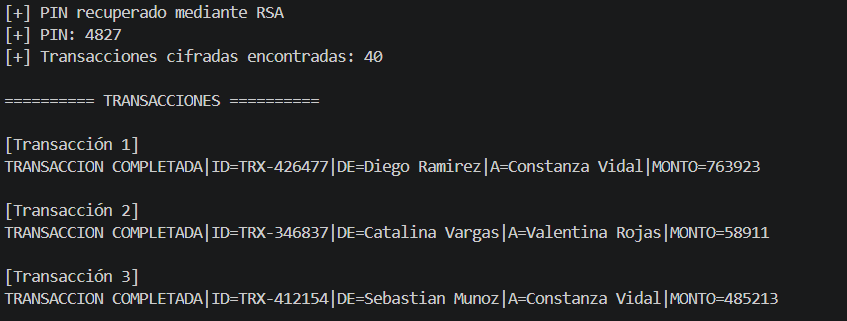
\includegraphics[width=0.86\textwidth]{img/figura1_ejemplo_guia.png}
    \caption{Ejemplo del resultado}
    \label{fig:ejemplo_resultado}
\end{figure}

Finalmente, responda la siguiente pregunta, justificando su respuesta: ¿Sería posible descifrar los mensajes capturados utilizando las claves pública y privada RSA en cifrados PQC (Criptografía post-cuántica)?

\newpage

% ==================== SECCIÓN 3: DESARROLLO DE ACTIVIDADES ====================
\section{Desarrollo de actividades}

\subsection{Actividad 1}

\subsubsection{Dockerfile}

Para desplegar un entorno aislado, reproducible y accesible desde la máquina anfitriona, se diseñó una imagen Docker basada en \texttt{ubuntu:22.04} con el servidor oficial \texttt{openssh-server} (OpenSSH 8.9p1). El proceso de construcción automatizado en \texttt{actividad\_1/Dockerfile} ejecuta secuencialmente las siguientes etapas:

\begin{enumerate}
    \item \textbf{Instalación no interactiva de paquetes:} Se define \texttt{ENV DEBIAN\_FRONTEND=noninteractive}, se actualizan los índices APT y se instalan \texttt{openssh-server}, \texttt{iproute2} y \texttt{net-tools}, limpiando posteriormente las listas temporales en \texttt{/var/lib/apt/lists/*} para minimizar la superficie de la imagen.
    \item \textbf{Preparación del entorno y claves del host:} Se crea el directorio de ejecución \texttt{/var/run/sshd} requerido por el demonio de separación de privilegios y se invoca \texttt{ssh-keygen -A} para generar el material criptográfico de host del servidor (incluyendo el par \texttt{/etc/ssh/ssh\_host\_ed25519\_key}).
    \item \textbf{Provisión de cuenta de prueba y validación sintáctica:} Se crea el usuario sin privilegios \texttt{usuario} con intérprete \texttt{/bin/bash} y contraseña conocida (\texttt{password123}) mediante \texttt{chpasswd}. Luego se copia el archivo \texttt{sshd\_config} endurecido a \texttt{/etc/ssh/sshd\_config}, se restringen sus permisos con \texttt{chmod 600} y se verifica su validez sintáctica durante el propio build con \texttt{/usr/sbin/sshd -t}.
    \item \textbf{Exposición y ejecución del servicio:} Se expone el puerto TCP \texttt{22} (\texttt{EXPOSE 22}) y se inicia \texttt{/usr/sbin/sshd -D -e} en primer plano. La imagen se construyó con \texttt{docker build -t ssh-lab4 actividad\_1/} y se levantó mapeando el puerto local \texttt{2222} hacia el puerto \texttt{22} del contenedor mediante \texttt{docker run -d -p 2222:22 --name servidor-ssh ssh-lab4}.
\end{enumerate}

El código fuente íntegro del archivo se encuentra disponible en GitHub en \href{https://github.com/minicoast/lab4-criptografia-udp/blob/main/actividad_1/Dockerfile}{\texttt{actividad\_1/Dockerfile}} (y el registro completo de construcción en \href{https://github.com/minicoast/lab4-criptografia-udp/blob/main/actividad_1/docker_build_log.txt}{\texttt{actividad\_1/docker\_build\_log.txt}}):

\begin{lstlisting}[language=bash,caption={Archivo \texttt{actividad\_1/Dockerfile} para el servidor OpenSSH.}]
FROM ubuntu:22.04

# Evitar prompts interactivos durante la instalación
ENV DEBIAN_FRONTEND=noninteractive

# Actualizar paquetes e instalar OpenSSH Server y utilidades de red
RUN apt-get update && \
    apt-get install -y openssh-server iproute2 net-tools && \
    rm -rf /var/lib/apt/lists/*

# Crear directorio de ejecución requerido por sshd
RUN mkdir -p /var/run/sshd

# Generar las claves del host SSH (incluyendo /etc/ssh/ssh_host_ed25519_key)
RUN ssh-keygen -A

# Crear usuario de prueba con contraseña conocida para la conexión SSH
RUN useradd -m -s /bin/bash usuario && \
    echo "usuario:password123" | chpasswd

# Copiar configuración personalizada con los algoritmos criptográficos exigidos
COPY sshd_config /etc/ssh/sshd_config
RUN chmod 600 /etc/ssh/sshd_config && /usr/sbin/sshd -t

# Exponer el puerto estándar SSH
EXPOSE 22

# Ejecutar el demonio sshd en primer plano
CMD ["/usr/sbin/sshd", "-D", "-e"]
\end{lstlisting}

\begin{figure}[H]
    \centering
    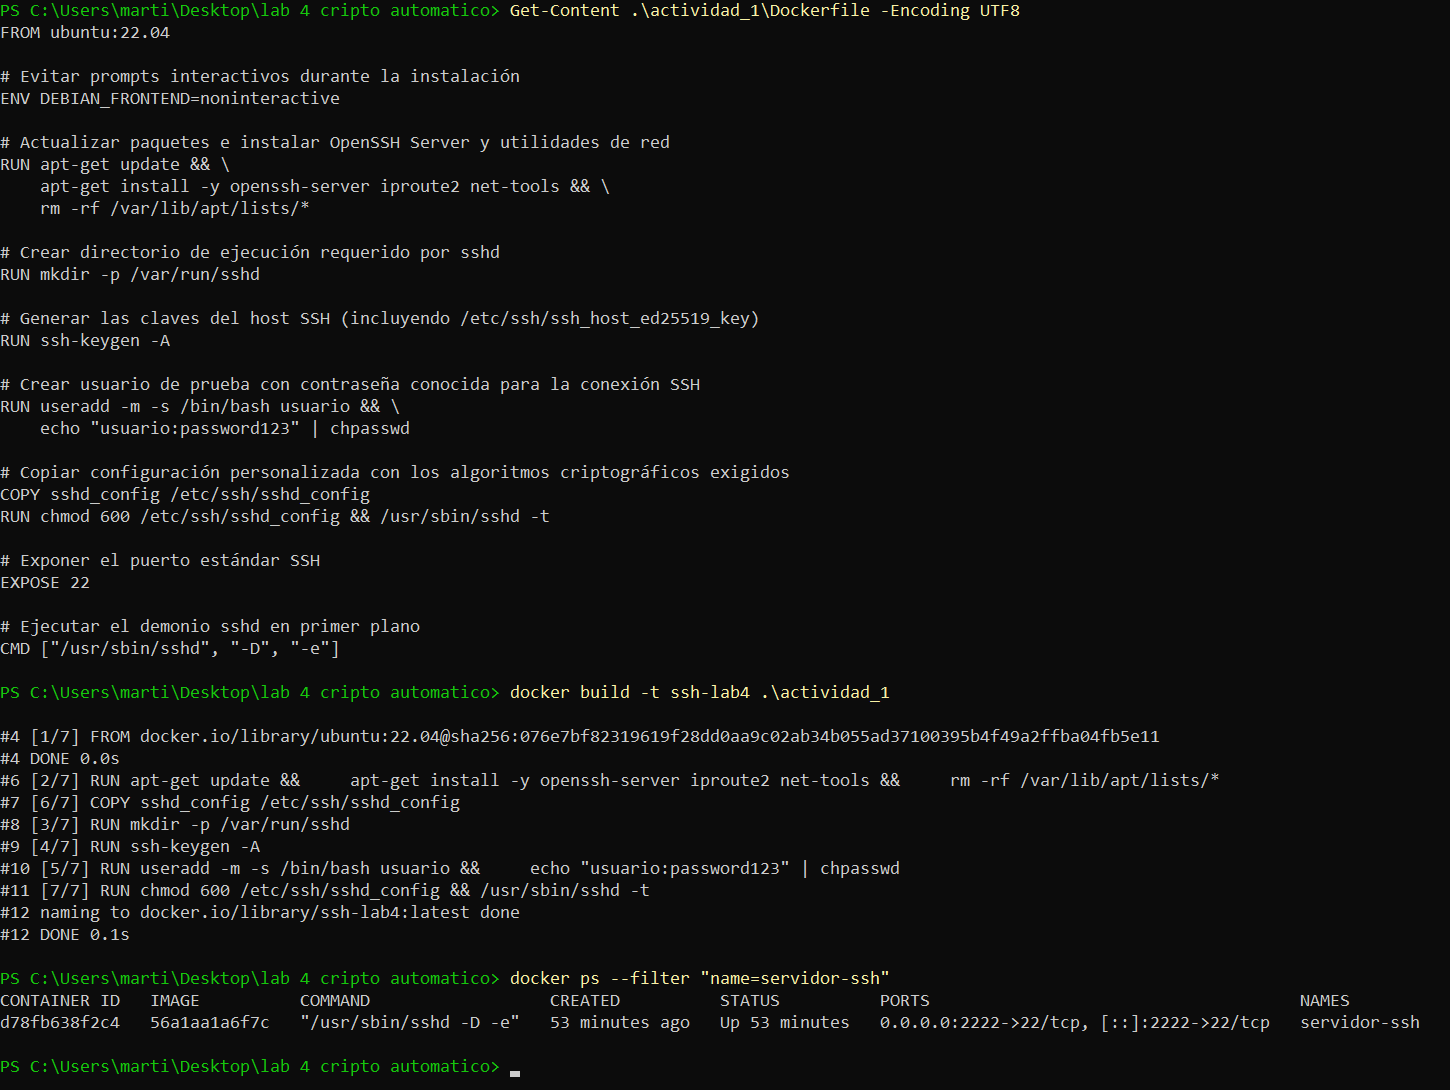
\includegraphics[width=0.98\textwidth]{img/01_dockerfile_build.png}
    \caption{Construcción de la imagen \texttt{ssh-lab4}, despliegue del contenedor \texttt{servidor-ssh} en el puerto \texttt{2222} y verificación con \texttt{docker ps}.}
    \label{fig:dockerfile_build}
\end{figure}

\subsubsection{Configuración del servidor}

Para restringir estrictamente la suite criptográfica del servidor OpenSSH a los algoritmos exigidos por la guía y eliminar cualquier mecanismo heredado o débil, se confeccionó el archivo \href{https://github.com/minicoast/lab4-criptografia-udp/blob/main/actividad_1/sshd_config}{\texttt{actividad\_1/sshd\_config}}. Las directivas clave aplicadas son:

\begin{itemize}
    \item \texttt{HostKey /etc/ssh/ssh\_host\_ed25519\_key}: instruye al demonio \texttt{sshd} a cargar únicamente la clave privada de host basada en curva Edwards25519.
    \item \texttt{KexAlgorithms curve25519-sha256}: fuerza como único mecanismo de intercambio de claves Diffie-Hellman sobre curva elíptica Curve25519 con función hash SHA-256.
    \item \texttt{Ciphers aes256-ctr}: restringe el cifrado simétrico del canal a AES con clave de 256 bits en modo contador (\textit{Counter Mode}).
    \item \texttt{MACs hmac-sha2-256}: exige autenticación e integridad de paquetes mediante HMAC basado en SHA-256.
    \item \texttt{HostKeyAlgorithms ssh-ed25519} y \texttt{PubkeyAcceptedAlgorithms ssh-ed25519}: obligan a utilizar firmas digitales Ed25519 tanto para autenticar la identidad del servidor como para claves públicas aceptadas.
    \item \texttt{PermitRootLogin no} y \texttt{PermitEmptyPasswords no}: deshabilitan el acceso directo como \texttt{root} y contraseñas vacías, habilitando \texttt{LogLevel VERBOSE} para auditoría detallada.
\end{itemize}

\begin{lstlisting}[language=bash,caption={Configuración endurecida en \texttt{actividad\_1/sshd\_config}.}]
# ========================================================
# Configuración Servidor OpenSSH - Laboratorio 4 Criptografía
# Algoritmos criptográficos forzados explícitamente:
#   - KexAlgorithms: curve25519-sha256
#   - Ciphers: aes256-ctr
#   - MACs: hmac-sha2-256
#   - HostKeyAlgorithms / PubkeyAcceptedAlgorithms: ssh-ed25519
# ========================================================

Port 22
ListenAddress 0.0.0.0

# Clave privada de host Ed25519
HostKey /etc/ssh/ssh_host_ed25519_key

# Algoritmos criptográficos requeridos por la guía y rúbrica
KexAlgorithms curve25519-sha256
Ciphers aes256-ctr
MACs hmac-sha2-256
HostKeyAlgorithms ssh-ed25519
PubkeyAcceptedAlgorithms ssh-ed25519

# Parámetros de autenticación y seguridad
PasswordAuthentication yes
PubkeyAuthentication yes
PermitEmptyPasswords no
PermitRootLogin no

# Nivel de registro y subsistema SFTP
LogLevel VERBOSE
Subsystem sftp /usr/lib/openssh/sftp-server
\end{lstlisting}

Una vez levantado el contenedor, se auditó la configuración efectiva en memoria ejecutando \texttt{docker exec servidor-ssh sshd -T}, comprobando que las cinco directivas criptográficas fueron aplicadas exactamente según lo requerido (Figura~\ref{fig:sshd_config}).

\begin{figure}[H]
    \centering
    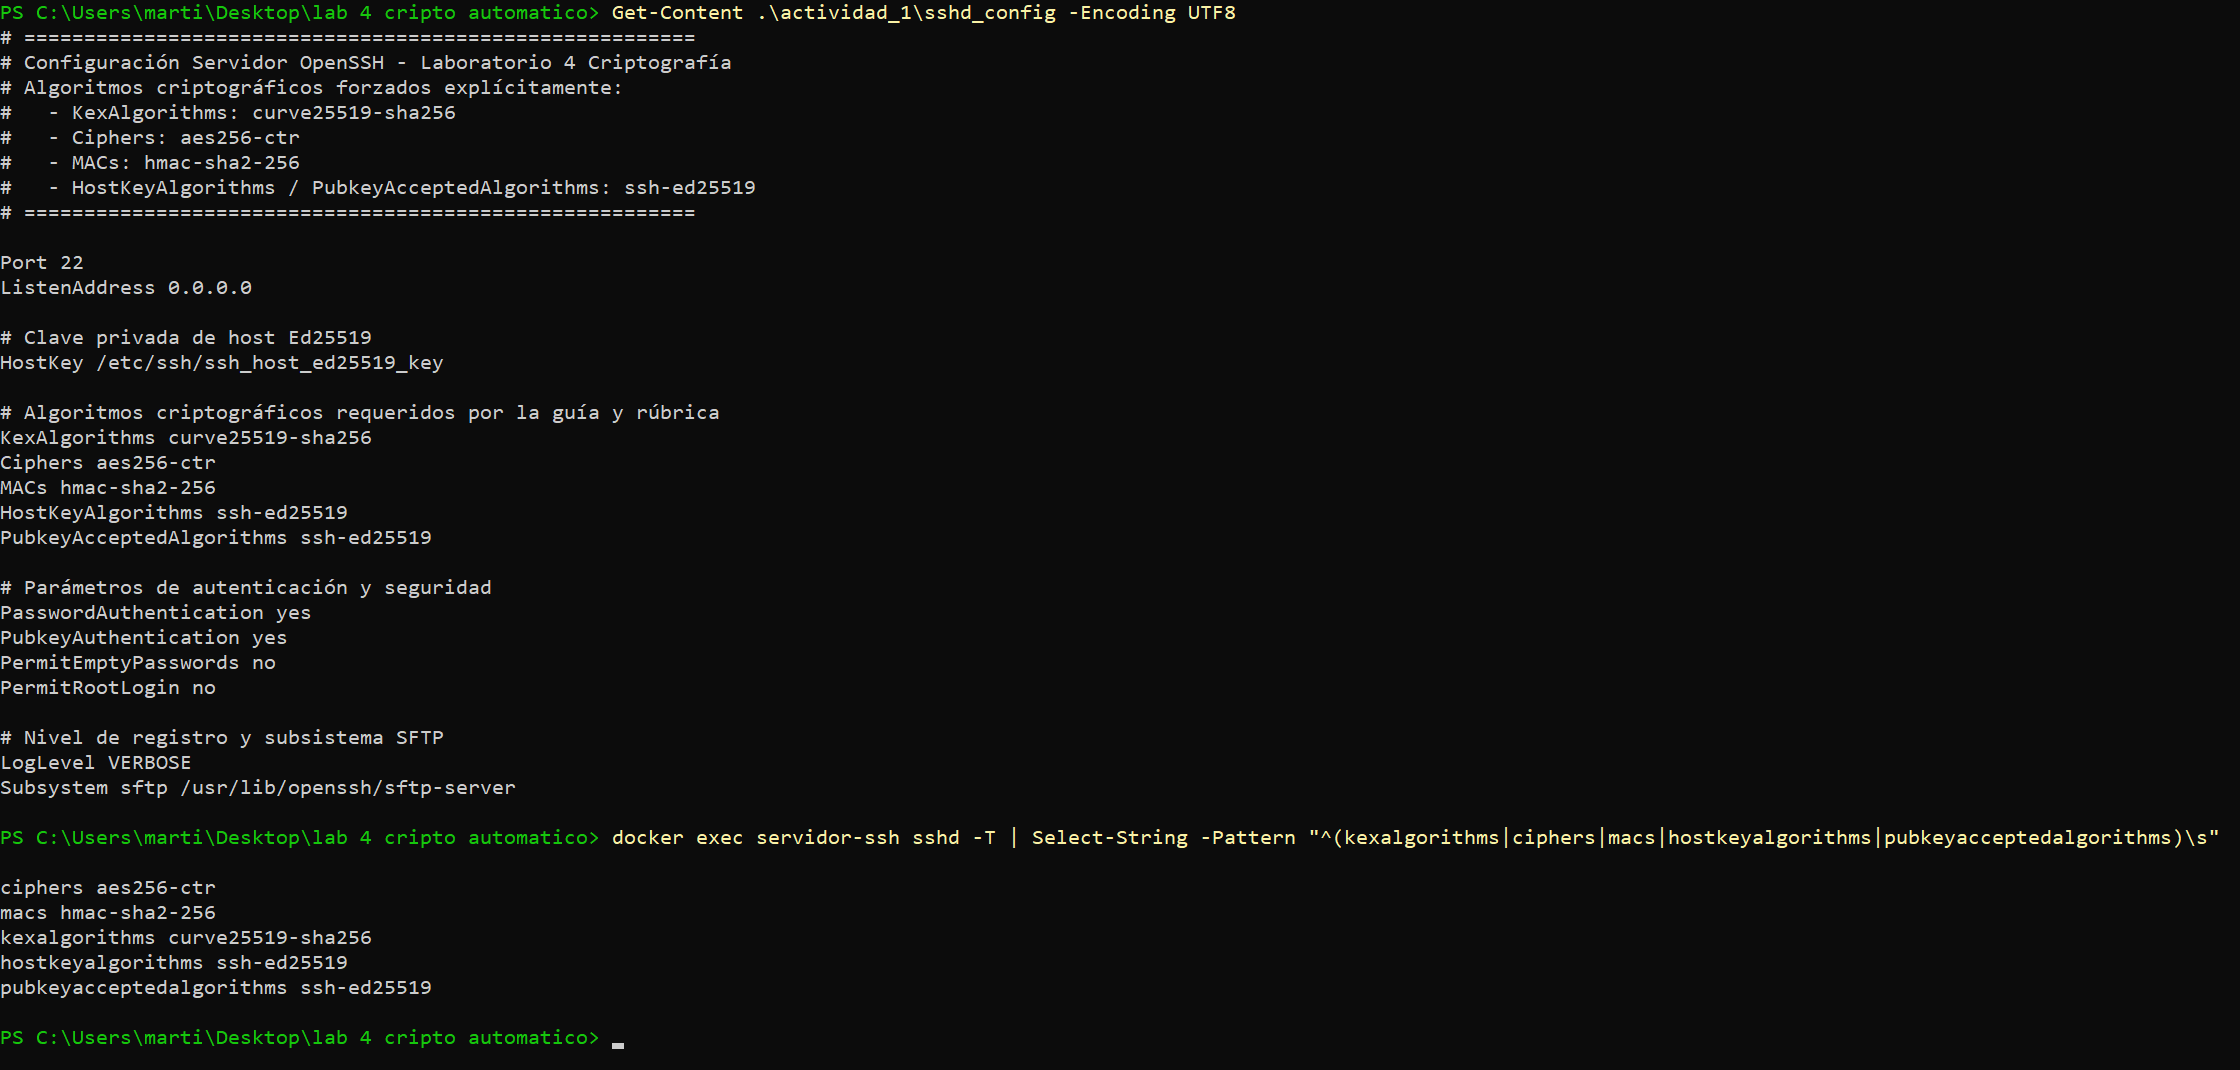
\includegraphics[width=0.98\textwidth]{img/02_sshd_config.png}
    \caption{Contenido de \texttt{sshd\_config} y verificación en tiempo de ejecución mediante \texttt{sshd -T} dentro del contenedor.}
    \label{fig:sshd_config}
\end{figure}

\subsubsection{Explicación de los algoritmos utilizados}

Dentro de la arquitectura del protocolo de transporte SSHv2 (RFC~4251 y RFC~4253), cada uno de los cuatro algoritmos configurados cumple una función de seguridad ortogonal e indispensable para proteger el establecimiento y la transmisión de datos:

\begin{enumerate}
    \item \textbf{\texttt{curve25519-sha256} (Intercambio de claves efímero — KEX y \textit{Perfect Forward Secrecy}):}
    Implementa el protocolo \textit{Elliptic Curve Diffie-Hellman} (ECDH / X25519, estandarizado para SSH en RFC~8731) sobre la curva de Montgomery $y^2 \equiv x^3 + 486662x^2 + x \pmod{2^{255}-19}$. Al iniciar la conexión, tanto el cliente como el servidor generan un par de claves efímeras de un solo uso $(a, Q_C = aG)$ y $(b, Q_S = bG)$, intercambiando únicamente las componentes públicas $Q_C$ y $Q_S$ de 32 bytes. Ambas partes calculan de manera independiente el mismo secreto compartido $K = aQ_S = bQ_C = abG$ en tiempo constante (mitigando ataques de canal lateral por temporización) y calculan el \textit{exchange hash} $H = \text{SHA-256}(V_C \parallel V_S \parallel I_C \parallel I_S \parallel K_S \parallel Q_C \parallel Q_S \parallel K)$. A partir de $K$ y $H$, SHA-256 deriva las claves simétricas direccionales de cifrado, los vectores de inicialización (IV) y las claves de integridad MAC. Debido a que las claves privadas efímeras $a$ y $b$ se destruyen de la memoria apenas finaliza el intercambio, este algoritmo garantiza \textbf{Secreto Perfecto hacia Adelante (\textit{Perfect Forward Secrecy}, PFS)}: incluso si la clave privada permanente del servidor fuese comprometida en el futuro, un atacante no podría descifrar sesiones capturadas previamente.

    \item \textbf{\texttt{aes256-ctr} (Cifrado simétrico de flujo — Confidencialidad):}
    Proporciona confidencialidad a todo el tráfico transmitido después del mensaje \texttt{SSH\_MSG\_NEWKEYS} (RFC~4344). Utiliza el estándar \textit{Advanced Encryption Standard} (AES) con clave simétrica de 256 bits (14 rondas de sustitución-permutación) operando en modo contador (\textit{Counter Mode}, CTR). En lugar de cifrar directamente los bloques de texto plano, AES cifra valores sucesivos de un contador de 128 bits inicializado con el IV derivado en KEX, produciendo un flujo pseudoaleatorio (\textit{keystream}) que se combina mediante XOR con el texto plano: $C_i = P_i \oplus E_{K_{\text{enc}}}(\text{CTR}_i)$. El modo CTR convierte un cifrador de bloques en un cifrador de flujo paralelizable y elimina vulnerabilidades históricas asociadas al modo CBC en SSH (como ataques de recuperación de texto plano contra encadenamiento de IVs predecibles).

    \item \textbf{\texttt{hmac-sha2-256} (Código de autenticación de mensajes — Integridad y autenticidad de paquetes):}
    Dado que \texttt{aes256-ctr} es un cifrado maleable que por sí solo garantiza confidencialidad pero no integridad, SSH complementa cada paquete con un \textit{Hash-based Message Authentication Code} basado en SHA-256 (RFC~6668). Para cada paquete transmitido con número de secuencia implícito de 32 bits $\text{seqnr}$, el emisor calcula:
    \[
        \begin{aligned}
        \text{MAC} &= \text{HMAC}_{K_{\text{mac}}}(\text{seqnr} \parallel \text{paquete\_en\_claro}) \\
                   &= \text{SHA-256}\!\Big((K_{\text{mac}} \oplus \text{opad}) \parallel \text{SHA-256}\big((K_{\text{mac}} \oplus \text{ipad}) \parallel \text{seqnr} \parallel M\big)\Big)
        \end{aligned}
    \]
    y adjunta la etiqueta resultante de 32 bytes (256 bits) al final del paquete cifrado. Esto garantiza simultáneamente \textbf{integridad de datos} (cualquier modificación de un solo bit en tránsito invalida el MAC), \textbf{autenticación de origen} (solo quien posee $K_{\text{mac}}$ puede generar etiquetas válidas) y \textbf{protección contra ataques de repetición o reordenamiento (\textit{replay})} gracias a la inclusión del contador monotónico $\text{seqnr}$.

    \item \textbf{\texttt{ssh-ed25519} (Esquema de firma digital de clave pública — Autenticación del servidor):}
    Implementa el algoritmo de firma digital \textit{Edwards-curve Digital Signature Algorithm} (EdDSA) sobre Edwards25519 con SHA-512 (RFC~8709). Un intercambio Diffie-Hellman anónimo sería vulnerable a ataques \textit{Man-in-the-Middle} (MitM) si un adversario activo interceptara $Q_C$ y $Q_S$. Para impedirlo, durante el paquete \texttt{SSH\_MSG\_KEX\_ECDH\_REPLY}, el servidor envía su clave pública permanente \texttt{ssh-ed25519} (32 bytes) junto con una firma digital $\sigma$ de 64 bytes calculada sobre el hash de intercambio $H$ usando su clave privada \texttt{/etc/ssh/ssh\_host\_ed25519\_key}. El cliente verifica criptográficamente $\sigma$ y contrasta la huella de la clave pública del servidor (\texttt{SHA256:E/jRjCqkaQh...}), autenticando sin ambigüedad la identidad del servidor y vinculando la sesión actual a dicho host. Además, Ed25519 genera sus nonces de firma de forma determinista mediante hash, eliminando fallos catastróficos por entropía débil propios de DSA/ECDSA tradicional.
\end{enumerate}

\begin{table}[H]
\centering
\caption{Resumen funcional de la suite criptográfica configurada en el servidor SSH.}
\label{tab:resumen_ssh_algs}
\resizebox{\textwidth}{!}{%
\begin{tabular}{@{}llll@{}}
\toprule
\textbf{Algoritmo} & \textbf{Categoría SSH} & \textbf{Propiedad de Seguridad} & \textbf{Fase donde Actúa} \\
\midrule
\texttt{curve25519-sha256} & Key Exchange (KEX) & Secreto compartido + PFS & Handshake inicial (ECDH) \\
\texttt{ssh-ed25519} & HostKey / Firma EdDSA & Autenticación de identidad (anti-MitM) & Respuesta \texttt{KEX\_ECDH\_REPLY} \\
\texttt{aes256-ctr} & Cifrado simétrico (256 b) & Confidencialidad de sesión & Túnel de datos post-\texttt{NEWKEYS} \\
\texttt{hmac-sha2-256} & MAC (256 b) & Integridad, autenticidad y anti-replay & Cada trama post-\texttt{NEWKEYS} \\
\bottomrule
\end{tabular}%
}
\end{table}

\subsubsection{Conexión cliente-servidor}

Mientras el capturador de paquetes se encontraba registrando el tráfico en la interfaz de loopback sobre el puerto TCP \texttt{2222}, se estableció la conexión desde la máquina cliente hacia el contenedor ejecutando \texttt{ssh -vv -o StrictHostKeyChecking=no -p 2222 usuario@127.0.0.1 "whoami \&\& hostname \&\& uname -a"}.

El modo de depuración extendido (\texttt{-vv}) permitió verificar en tiempo real que el cliente recibió la propuesta restringida del servidor (\texttt{peer server KEXINIT proposal}) y seleccionó exactamente los cuatro algoritmos configurados: \texttt{kex: algorithm: curve25519-sha256}, \texttt{kex: host key algorithm: ssh-ed25519}, \texttt{cipher: aes256-ctr} y \texttt{MAC: hmac-sha2-256} en ambas direcciones (\texttt{server->client} y \texttt{client->server}). Tras validar la clave pública Ed25519 del contenedor y activar las claves simétricas con \texttt{SSH2\_MSG\_NEWKEYS}, se completó la autenticación de usuario y se ejecutaron remotamente los comandos diagnósticos retornando \texttt{usuario}, el identificador del contenedor \texttt{d78fb638f2c4} y el kernel Linux subyacente con código de salida \texttt{0} (Figura~\ref{fig:ssh_cliente}). El registro íntegro de 152 líneas se encuentra respaldado en \href{https://github.com/minicoast/lab4-criptografia-udp/blob/main/actividad_1/ssh_vv_completo.log}{\texttt{actividad\_1/ssh\_vv\_completo.log}}.

\begin{figure}[H]
    \centering
    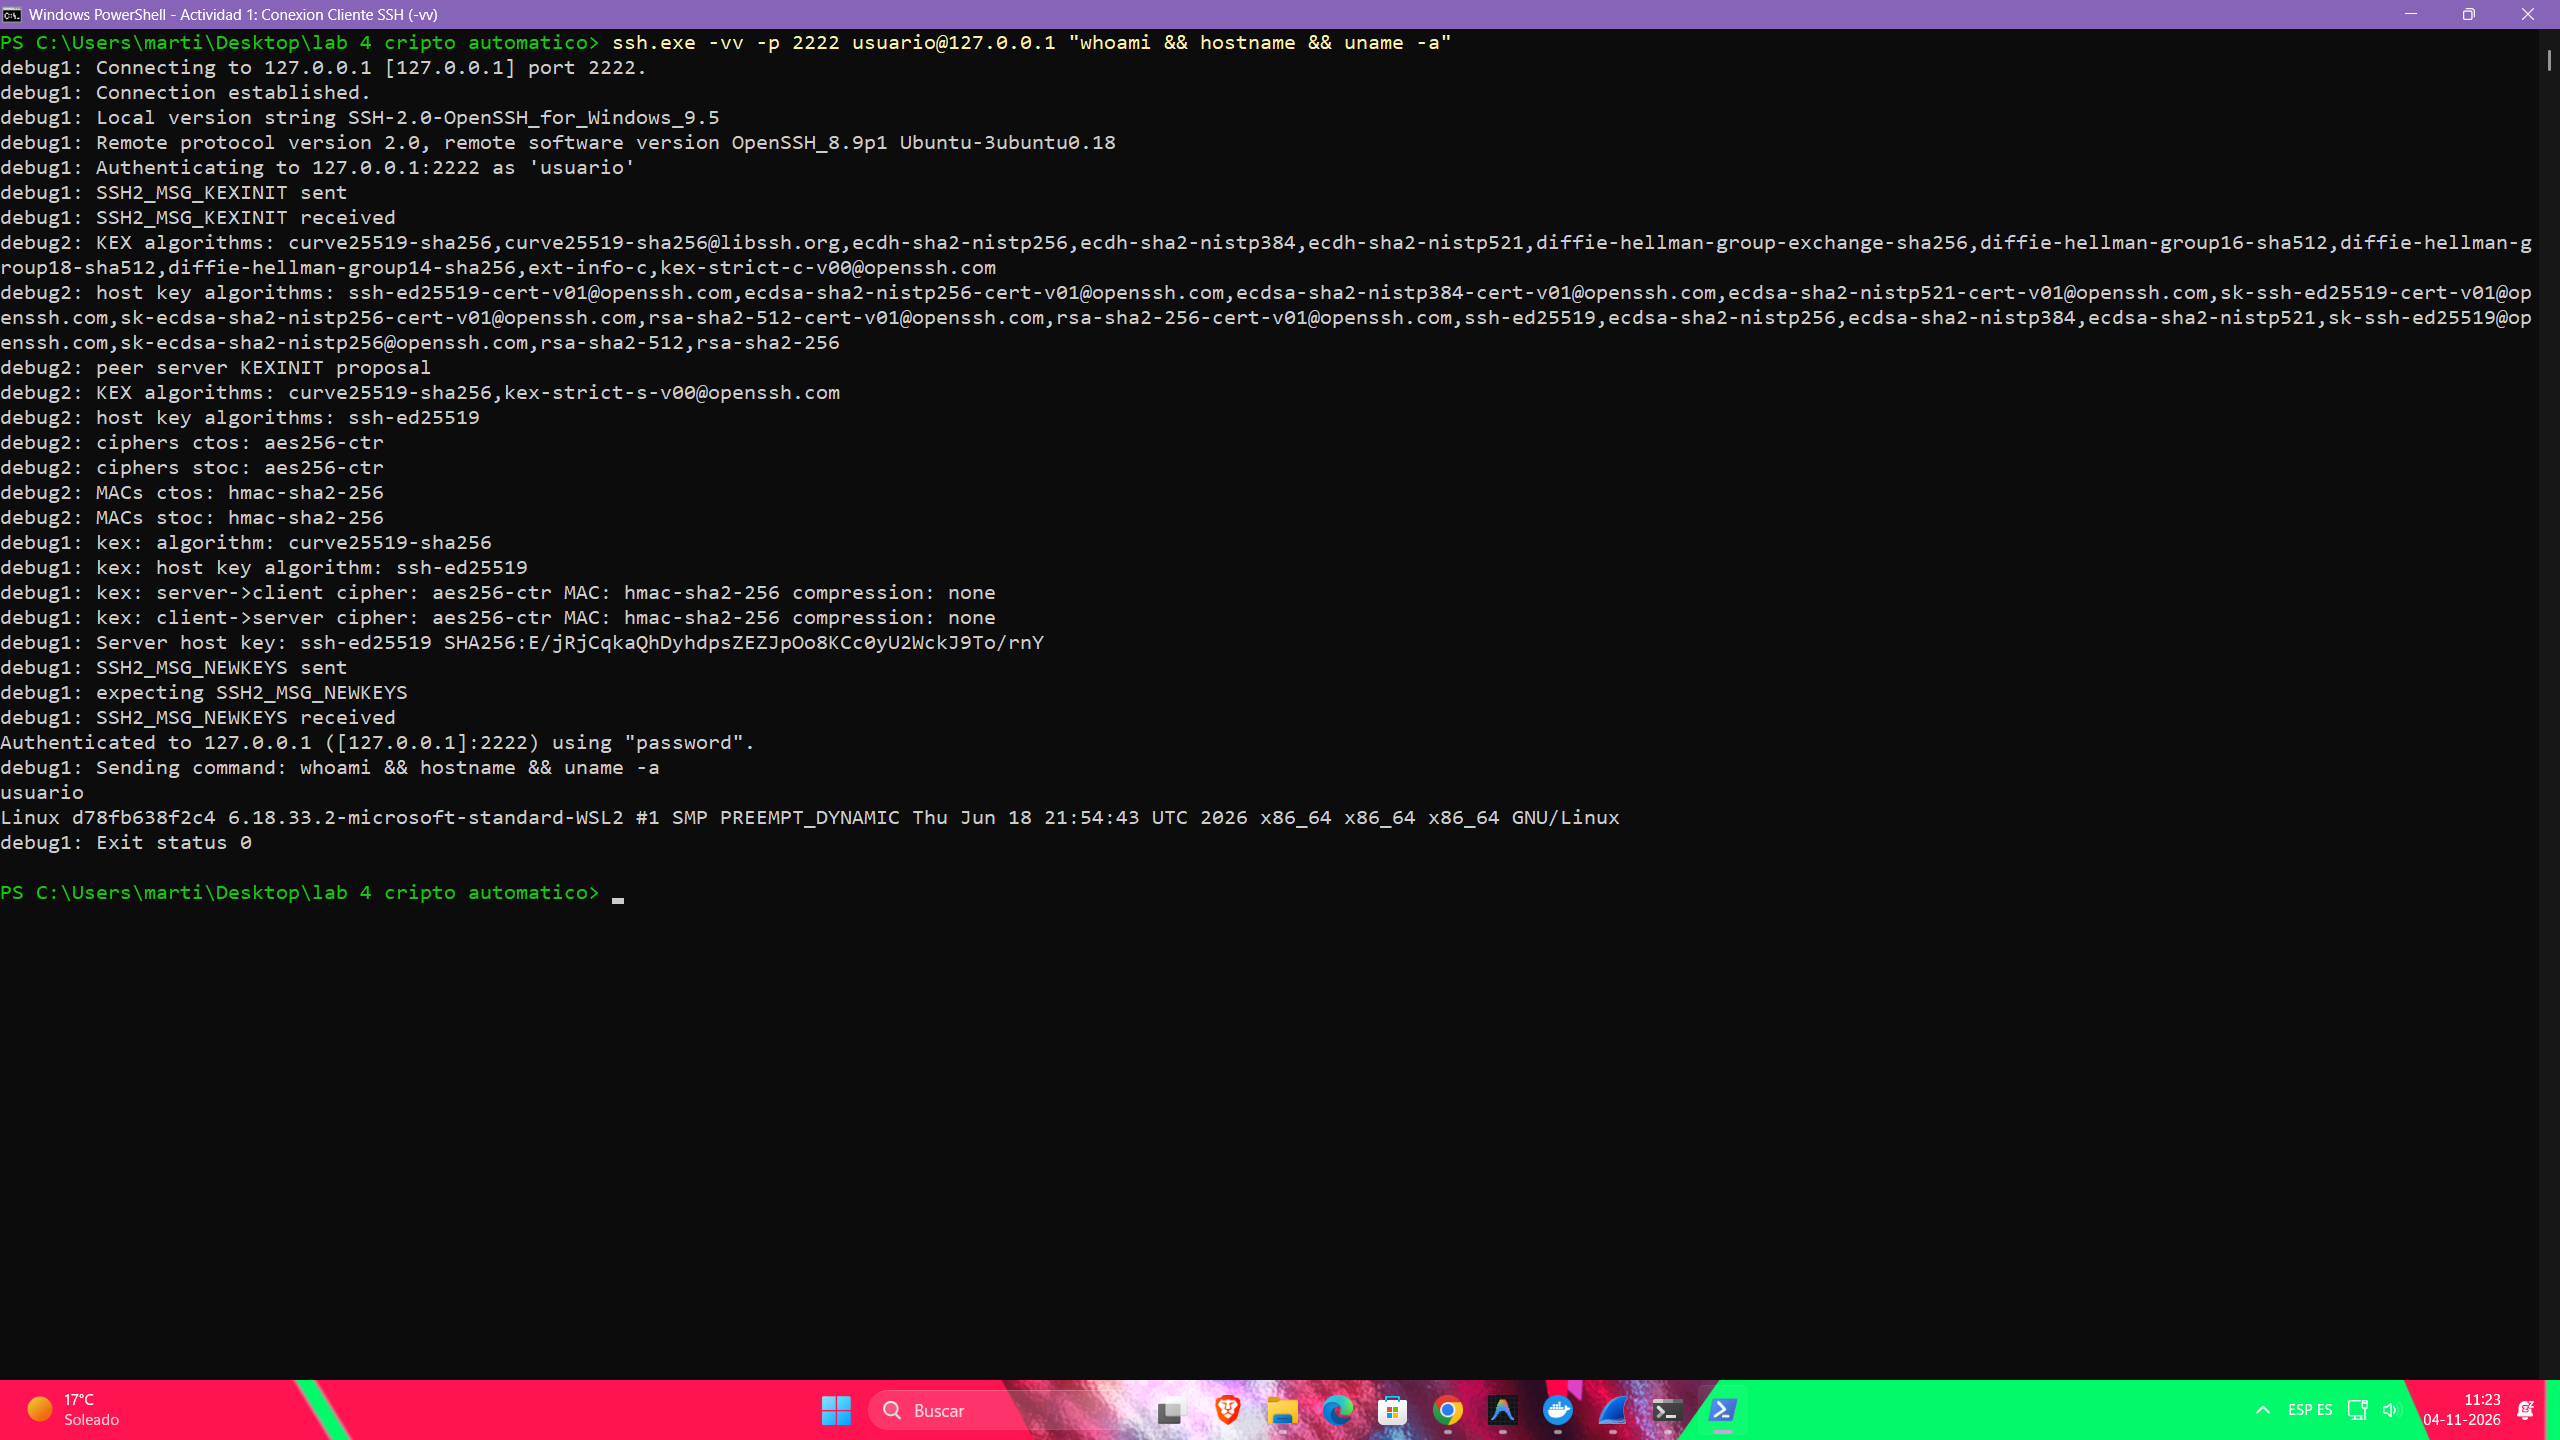
\includegraphics[width=0.98\textwidth]{img/03_ssh_conexion_cliente.png}
    \caption{Conexión exitosa del cliente \texttt{ssh -vv} negociando los cuatro algoritmos configurados y ejecutando comandos dentro del contenedor Docker.}
    \label{fig:ssh_cliente}
\end{figure}

\subsubsection{Análisis de tráfico}

El tráfico completo de la sesión (56 tramas TCP/SSHv2) fue capturado en formato \texttt{.pcap} en \href{https://github.com/minicoast/lab4-criptografia-udp/blob/main/actividad_1/captura_ssh.pcap}{\texttt{actividad\_1/\allowbreak captura\_ssh.pcap}} y desglosado mediante Wireshark/\texttt{tshark} en el archivo \href{https://github.com/minicoast/lab4-criptografia-udp/blob/main/actividad_1/analisis_wireshark_ssh.txt}{\texttt{actividad\_1/\allowbreak analisis\_wireshark\_ssh.txt}} (Figura~\ref{fig:wireshark_ssh}).

\begin{figure}[H]
    \centering
    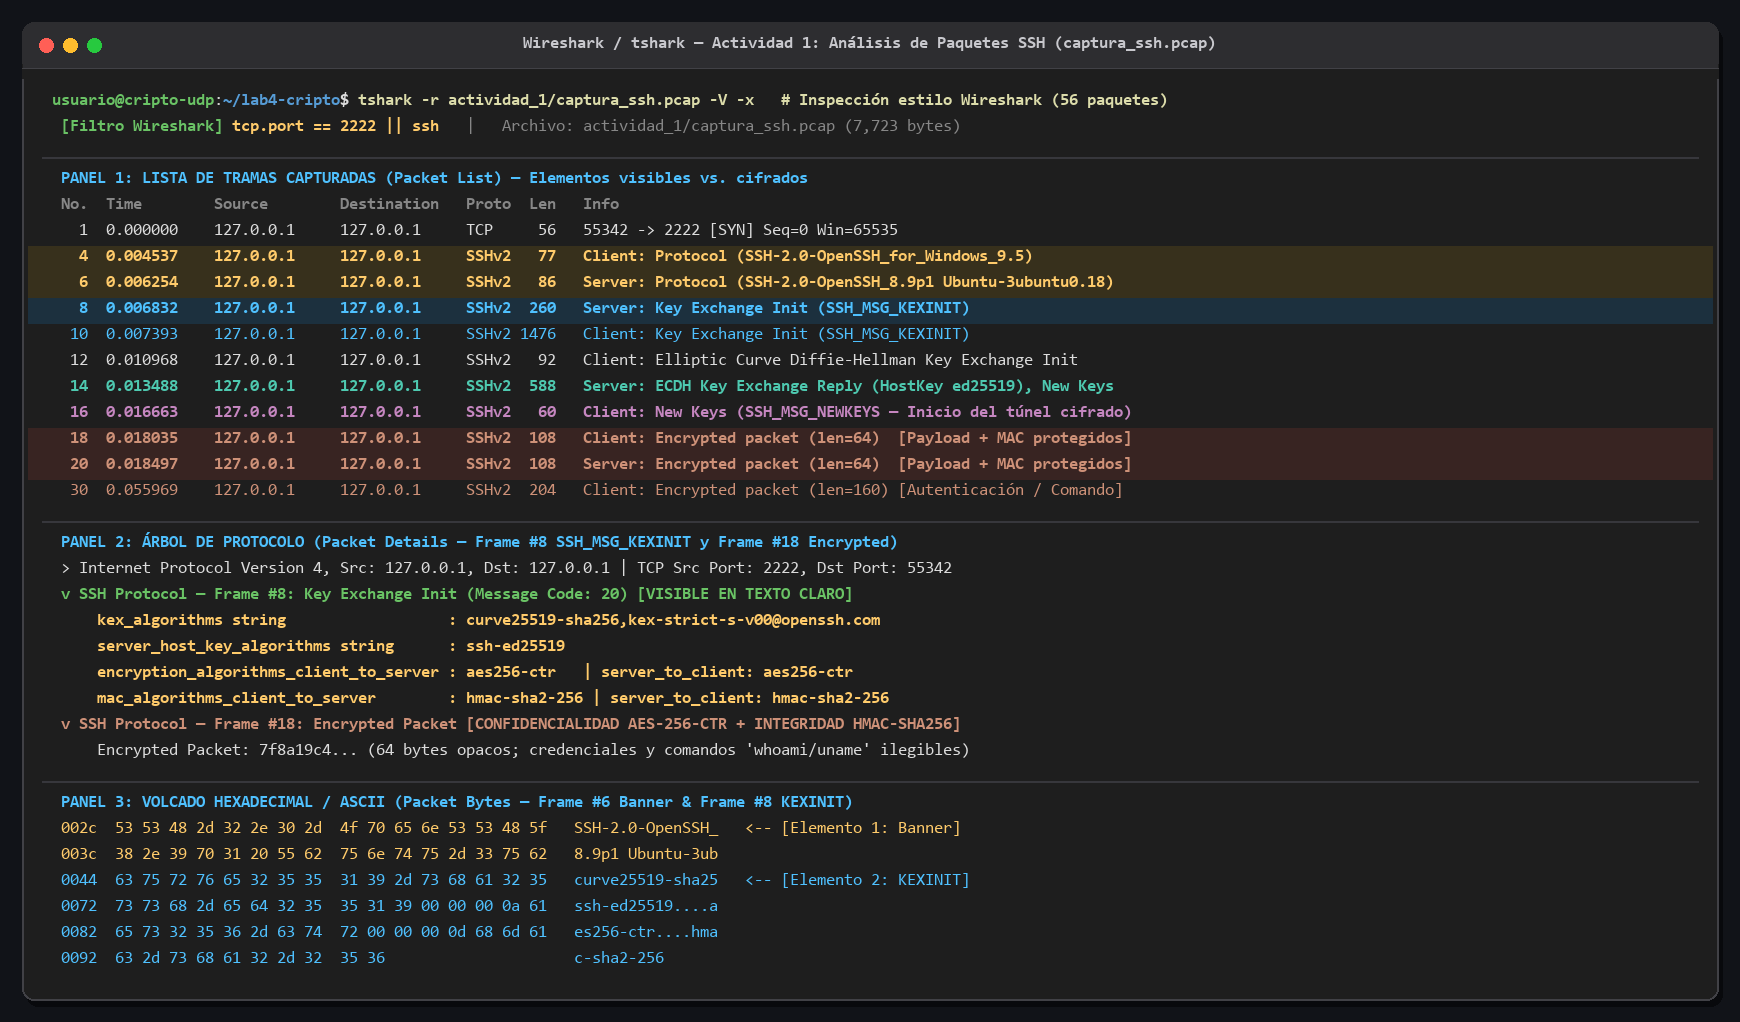
\includegraphics[width=0.99\textwidth]{img/04_wireshark_ssh.png}
    \caption{Inspección de paquetes SSH en Wireshark/\texttt{tshark} sobre \texttt{captura\_ssh.pcap}: lista de tramas, árbol de protocolo y volcado hexadecimal.}
    \label{fig:wireshark_ssh}
\end{figure}

\noindent\textbf{Respuesta a la pregunta de análisis: ¿Qué información es posible identificar a partir de los paquetes capturados?}

Un tercero con acceso pasivo al tráfico de red (\textit{eavesdropper}) \textbf{no puede leer credenciales ni comandos}, pero sí puede observar en texto claro diversos metadatos de red y parámetros de negociación previos a la activación del cifrado. A partir de los paquetes capturados se identifican claramente los siguientes \textbf{cuatro elementos observables}:

\begin{enumerate}
    \item \textbf{Banners con versión de protocolo, software exacto y sistema operativo (Frames \#4 y \#6):}
    Inmediatamente después del \textit{three-way handshake} TCP (Frames \#1--\#3), tanto cliente como servidor intercambian cadenas ASCII legibles sin cifrar. En el Frame \#4 se lee literalmente \texttt{SSH-2.0-OpenSSH\_for\_Windows\_9.5} y en el Frame \#6 \texttt{SSH-2.0-OpenSSH\_8.9p1 Ubuntu-3ubuntu0.18}. Esto revela a un observador externo que se utiliza SSHv2, las implementaciones exactas de cliente y servidor e incluso la distribución y nivel de parche del sistema operativo anfitrión (\textit{banner grabbing}), información valiosa durante fases de reconocimiento para buscar vulnerabilidades conocidas (CVEs).

    \item \textbf{Listas completas de algoritmos criptográficos soportados y negociados en \texttt{SSH\_MSG\_KEXINIT} (Frames \#8 y \#10):}
    Los paquetes con código de mensaje \texttt{20} (\textit{Key Exchange Init}) viajan íntegramente en texto plano. Al expandir el Frame \#8 del servidor se leen en ASCII claro las cadenas \texttt{curve25519-sha256}, \texttt{ssh-ed25519}, \texttt{aes256-ctr}, \texttt{hmac-sha2-256} y \texttt{none,zlib@openssh.com}, junto con la \textit{cookie} aleatoria de 16 bytes (\texttt{45ffb830...}) y la huella \textit{HASSH} del servidor (\texttt{2fac0554777f542556a28eca6854f64b}). Un tercero puede así auditar la postura criptográfica de ambos extremos y detectar si algún servidor acepta cifradores obsoletos.

    \item \textbf{Claves públicas efímeras ECDH, clave pública permanente del host y señalización \texttt{SSH\_MSG\_NEWKEYS} (Frames \#12, \#14 y \#16):}
    En el Frame \#12 (\texttt{Elliptic Curve Diffie-Hellman Key Exchange Init}) es visible la clave pública efímera $Q_C$ de 32 bytes del cliente, y en el Frame \#14 (\texttt{Key Exchange Reply}) se observan la clave pública efímera $Q_S$ del servidor, su clave pública permanente \texttt{ssh-ed25519} y la firma EdDSA sobre el hash $H$. Seguidamente, el código de mensaje \texttt{21} (\texttt{New Keys}, Frame \#16) indica explícitamente el punto exacto donde ambos extremos activan las claves derivadas.

    \item \textbf{Metadatos de transporte TCP/IP y patrones de longitud/temporización de \texttt{Encrypted packet} (Frames \#1 al \#56):}
    Durante toda la comunicación permanecen visibles las cabeceras IP y TCP: direcciones IP origen y destino (\texttt{127.0.0.1}), puerto efímero del cliente (\texttt{55342}) y puerto del servicio (\texttt{2222}), banderas TCP, marcas de tiempo y tamaños exactos de cada trama \texttt{Encrypted packet (len=64)}, \texttt{(len=80)}, \texttt{(len=160)}, \texttt{(len=256)}, permitiendo inferir duración de la sesión, volumen total transferido y si se trata de escritura interactiva tecla a tecla o ejecución por lotes.
\end{enumerate}

\noindent\textbf{Elementos protegidos mediante cifrado:} A partir del Frame \#18 en adelante (tras \texttt{SSH\_MSG\_NEWKEYS}), toda la carga útil de aplicación aparece encapsulada exclusivamente como \texttt{Encrypted packet}. Gracias a \texttt{aes256-ctr} y \texttt{hmac-sha2-256}, permanecen completamente confidenciales e íntegros el nombre de usuario (\texttt{usuario}), el método y la contraseña de autenticación (\texttt{password123} dentro de \texttt{ssh-userauth}), los comandos ejecutados (\texttt{whoami \&\& hostname \&\& uname -a}), la salida estándar devuelta por el contenedor y cualquier archivo o flujo transferido.

\subsection{Actividad 2}

\subsubsection{Identificación del paquete RSA\_PIN}

Para inspeccionar sistemáticamente la captura histórica \href{https://github.com/minicoast/lab4-criptografia-udp/blob/main/transacciones_cifradas.pcap}{\texttt{transacciones\_cifradas.pcap}}, se desarrolló el script \href{https://github.com/minicoast/lab4-criptografia-udp/blob/main/actividad_2/analizar_pcap.py}{\texttt{actividad\_2/analizar\_pcap.py}}, el cual analiza las cabeceras IP/TCP y exporta los volcados hexadecimales completos en \href{https://github.com/minicoast/lab4-criptografia-udp/blob/main/actividad_2/hexdump_paquetes.txt}{\texttt{actividad\_2/hexdump\_paquetes.txt}}.

La captura consta de exactamente \textbf{41 tramas TCP} transmitidas desde \texttt{10.10.10.10:49152} hacia \texttt{10.10.10.20:4444}. El \textbf{Paquete \#1} (320 bytes en cable; 280 bytes de carga útil TCP) corresponde al paquete de inicialización criptográfica identificado por el prefijo ASCII \texttt{RSA\_PIN|}, cuya estructura interna de 280 bytes se descompone de la siguiente manera (Figura~\ref{fig:paquete_rsa_pin}):

\begin{itemize}
    \item \textbf{Bytes \texttt{[0x0000 -- 0x0007]} (8 bytes):} Etiqueta identificadora en ASCII \texttt{RSA\_PIN|} (\texttt{52 53 41 5f 50 49 4e 7c}).
    \item \textbf{Bytes \texttt{[0x0008 -- 0x0017]} (16 bytes / 128 bits):} Valor de \texttt{salt} aleatorio en binario crudo (\texttt{1a065da01a70284041b93dd58e988907}) requerido posteriormente por la función derivadora \texttt{Scrypt}.
    \item \textbf{Bytes \texttt{[0x0018 -- 0x0117]} (256 bytes / 2048 bits):} Criptograma asimétrico RSA-2048 generado mediante relleno óptimo OAEP con SHA-256 (\texttt{2e94beb47c1f4ffd...\allowbreak c1c97831a5faa6de}), cuyo tamaño coincide exactamente con el módulo de 2048 bits (256 bytes) de \href{https://github.com/minicoast/lab4-criptografia-udp/blob/main/clave_publica.pem}{\texttt{clave\_publica.pem}}.
\end{itemize}

\begin{figure}[H]
    \centering
    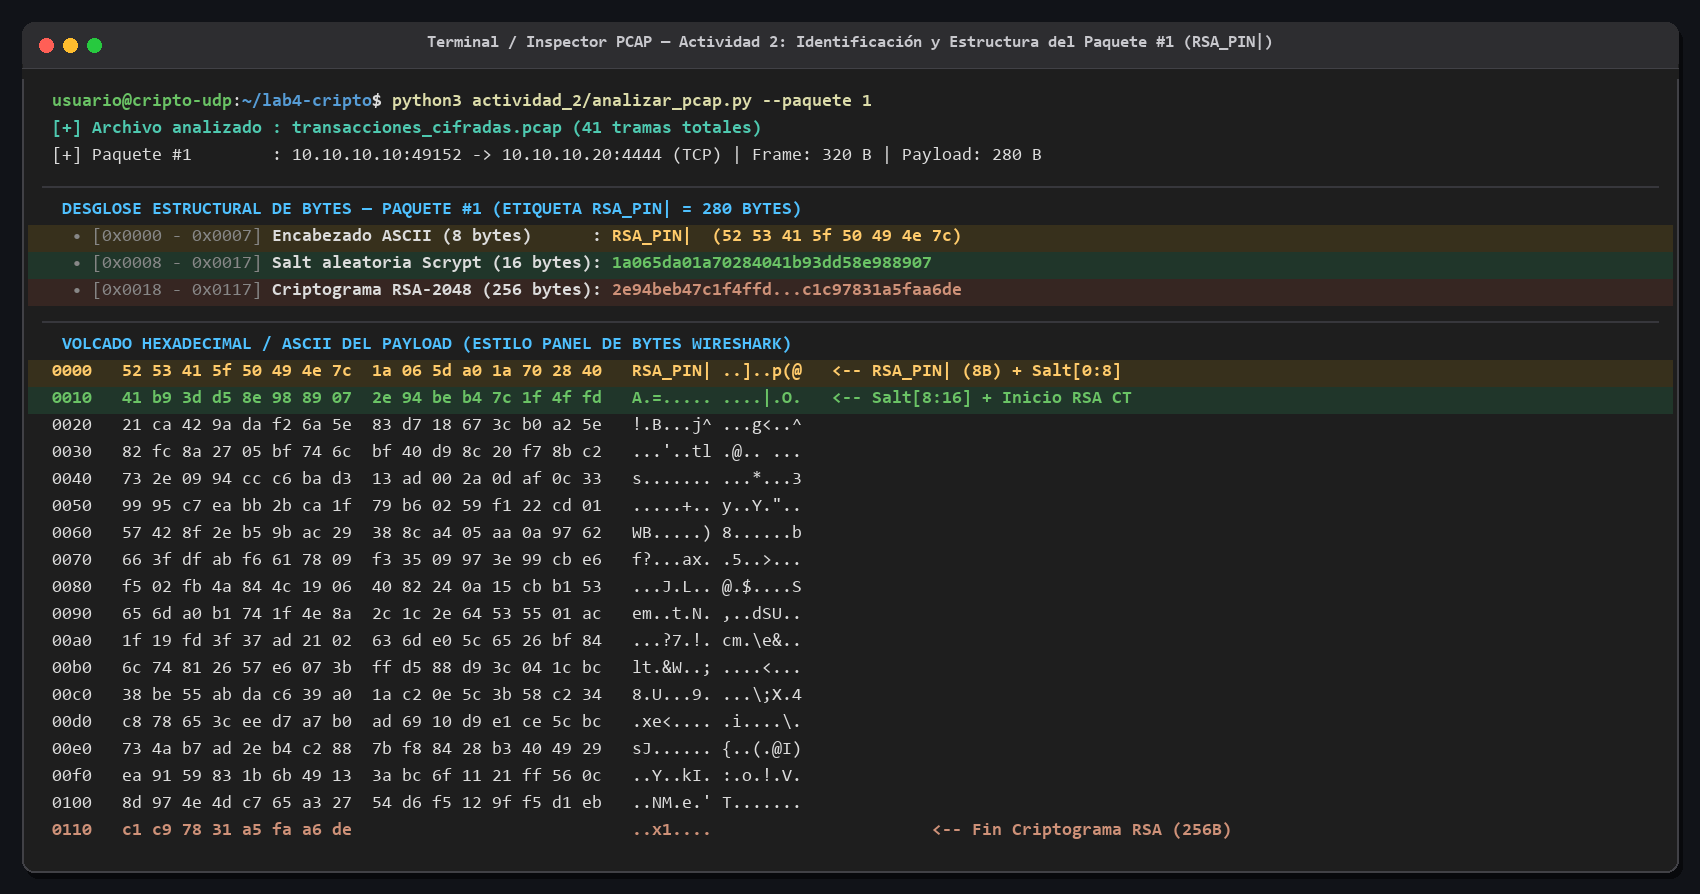
\includegraphics[width=0.98\textwidth]{img/05_paquete_rsa_pin.png}
    \caption{Identificación estructural y volcado hexadecimal/ASCII del Paquete \#1 (\texttt{RSA\_PIN|}) en \texttt{transacciones\_cifradas.pcap}.}
    \label{fig:paquete_rsa_pin}
\end{figure}

\subsubsection{Identificación de los paquetes AESGCM}

Las \textbf{40 tramas restantes} de la captura (Frames \#2 al \#41, con cargas útiles TCP entre 116 y 121 bytes) presentan todas el encabezado en claro \texttt{AESGCM|} (\texttt{41 45 53 47 43 4d 7c}), confirmando la presencia de exactamente \textbf{40 transacciones financieras cifradas} mediante el esquema de cifrado autenticado con datos asociados (\textit{AEAD}) \textbf{AES-256-GCM} (NIST SP 800-38D). El desglose exacto de bytes de cada paquete es el siguiente (Figura~\ref{fig:paquetes_aesgcm}, respaldo completo en \href{https://github.com/minicoast/lab4-criptografia-udp/blob/main/actividad_2/hexdump_paquetes.txt}{\texttt{actividad\_2/hexdump\_paquetes.txt}}):

\begin{itemize}
    \item \textbf{Bytes \texttt{[0x0000 -- 0x0006]} (7 bytes):} Prefijo de protocolo \texttt{AESGCM|}.
    \item \textbf{Bytes \texttt{[0x0007 -- 0x0012]} (12 bytes / 96 bits):} \texttt{Nonce} único por mensaje (estándar de 96 bits recomendado por NIST para GCM; por ejemplo, \texttt{2f0f7c0cec6fc6216066c11e} en el Frame \#2). Se verificó que los 40 paquetes emplean 40 \textit{nonces} distintos, evitando la reutilización de flujo CTR y preservando la seguridad de GHASH.
    \item \textbf{Bytes \texttt{[0x0013 -- N-17]} (81 a 86 bytes):} Texto cifrado (\textit{ciphertext}) de longitud idéntica al mensaje original en UTF-8.
    \item \textbf{Últimos 16 bytes \texttt{[N-16 -- N-1]} (16 bytes / 128 bits):} Etiqueta de autenticación criptográfica (\textit{GCM Authentication Tag}) adjuntada al final del criptograma por la biblioteca \texttt{cryptography}, utilizada para verificar integridad y autenticidad antes de liberar cualquier byte descifrado.
\end{itemize}

\begin{figure}[H]
    \centering
    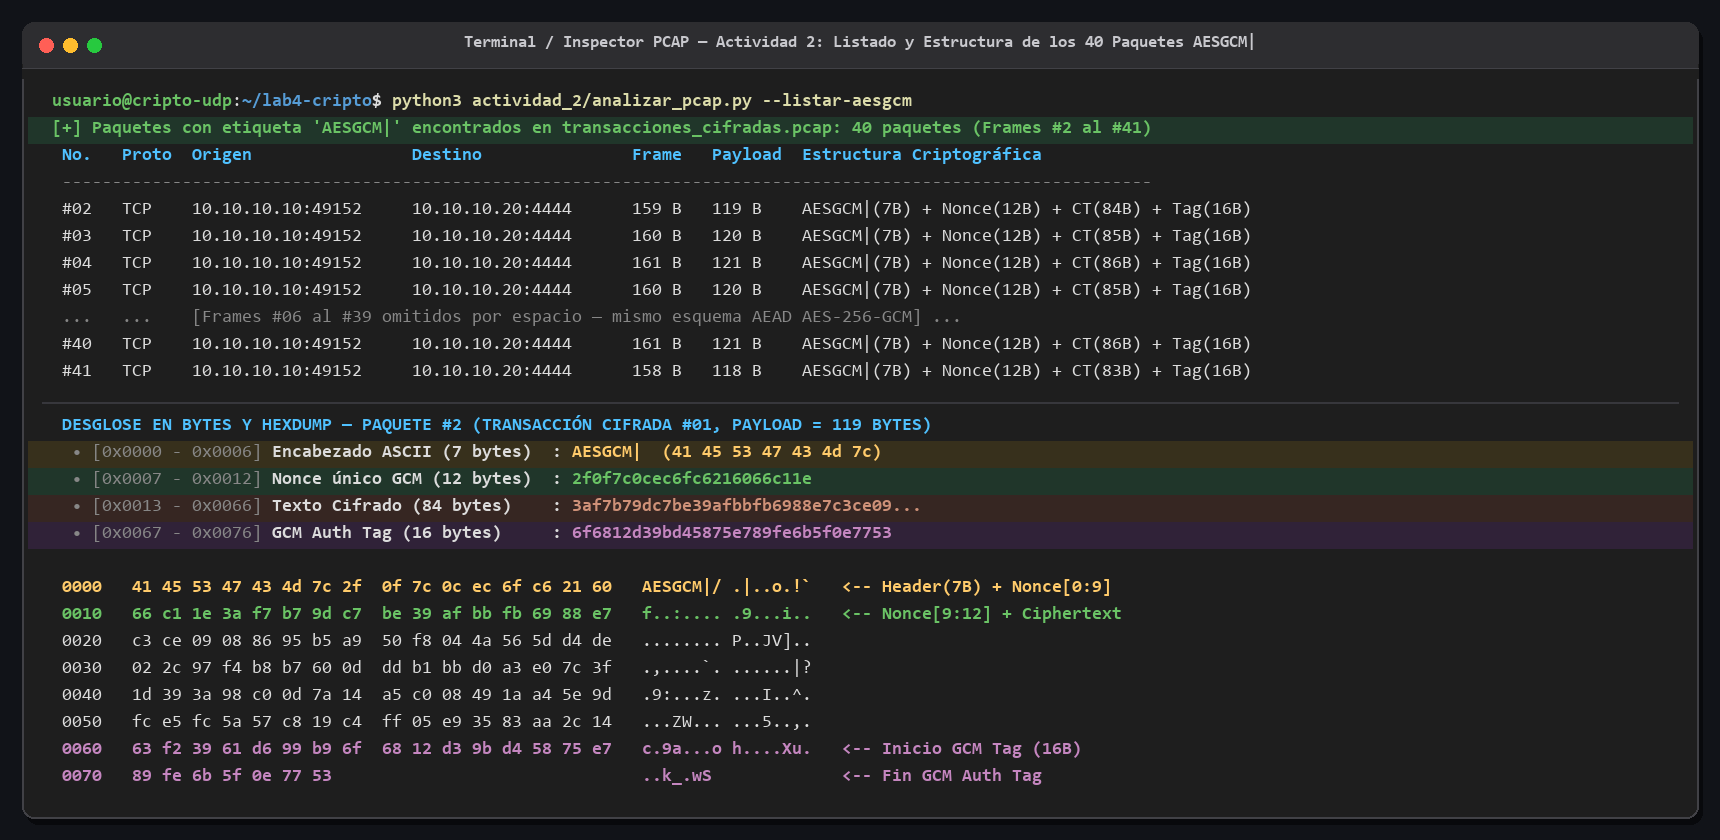
\includegraphics[width=0.98\textwidth]{img/06_paquetes_aesgcm.png}
    \caption{Listado de los 40 paquetes \texttt{AESGCM|} encontrados y desglose hexadecimal de \texttt{nonce}, texto cifrado y etiqueta GCM.}
    \label{fig:paquetes_aesgcm}
\end{figure}

\subsubsection{Recuperación del PIN y derivación de la clave AES}

A partir de los campos extraídos del Paquete \#1 y utilizando la clave privada RSA-2048 proporcionada (\href{https://github.com/minicoast/lab4-criptografia-udp/blob/main/clave_privada.pem}{\texttt{clave\_privada.pem}}), se ejecutó la fase de recuperación del secreto y derivación simétrica en dos pasos (Figura~\ref{fig:pin_scrypt}):

\begin{enumerate}
    \item \textbf{Descifrado asimétrico RSA-OAEP con SHA-256:} Se cargó \texttt{clave\_privada.pem} mediante \texttt{serialization.\allowbreak load\_pem\_private\_key()} y se descifró el bloque de 256 bytes invocando \texttt{private\_key.decrypt()} con el esquema de relleno \texttt{padding.OAEP(\allowbreak mgf=padding.MGF1(hashes.SHA256()), \allowbreak algorithm=hashes.SHA256(), \allowbreak label=None)}. La operación validó satisfactoriamente la estructura OAEP y recuperó el PIN de 4 dígitos en texto claro: \textbf{\texttt{4827}}.
    \item \textbf{Derivación de clave simétrica de 256 bits con Scrypt:} Se instanció \texttt{Scrypt(salt=salt, length=32, n=2**14, r=8, p=1)} alimentando \texttt{kdf.derive(b"4827")} junto con la \texttt{salt} extraída (\texttt{1a065da01a70284041b93dd58e988907}), obteniendo la clave AES de 32 bytes (256 bits):\\
    \texttt{f64d739ad8bd559fcd4bde7b9aecb83ff28d200331da635d7409b7133b16eab7}.
\end{enumerate}

\begin{figure}[H]
    \centering
    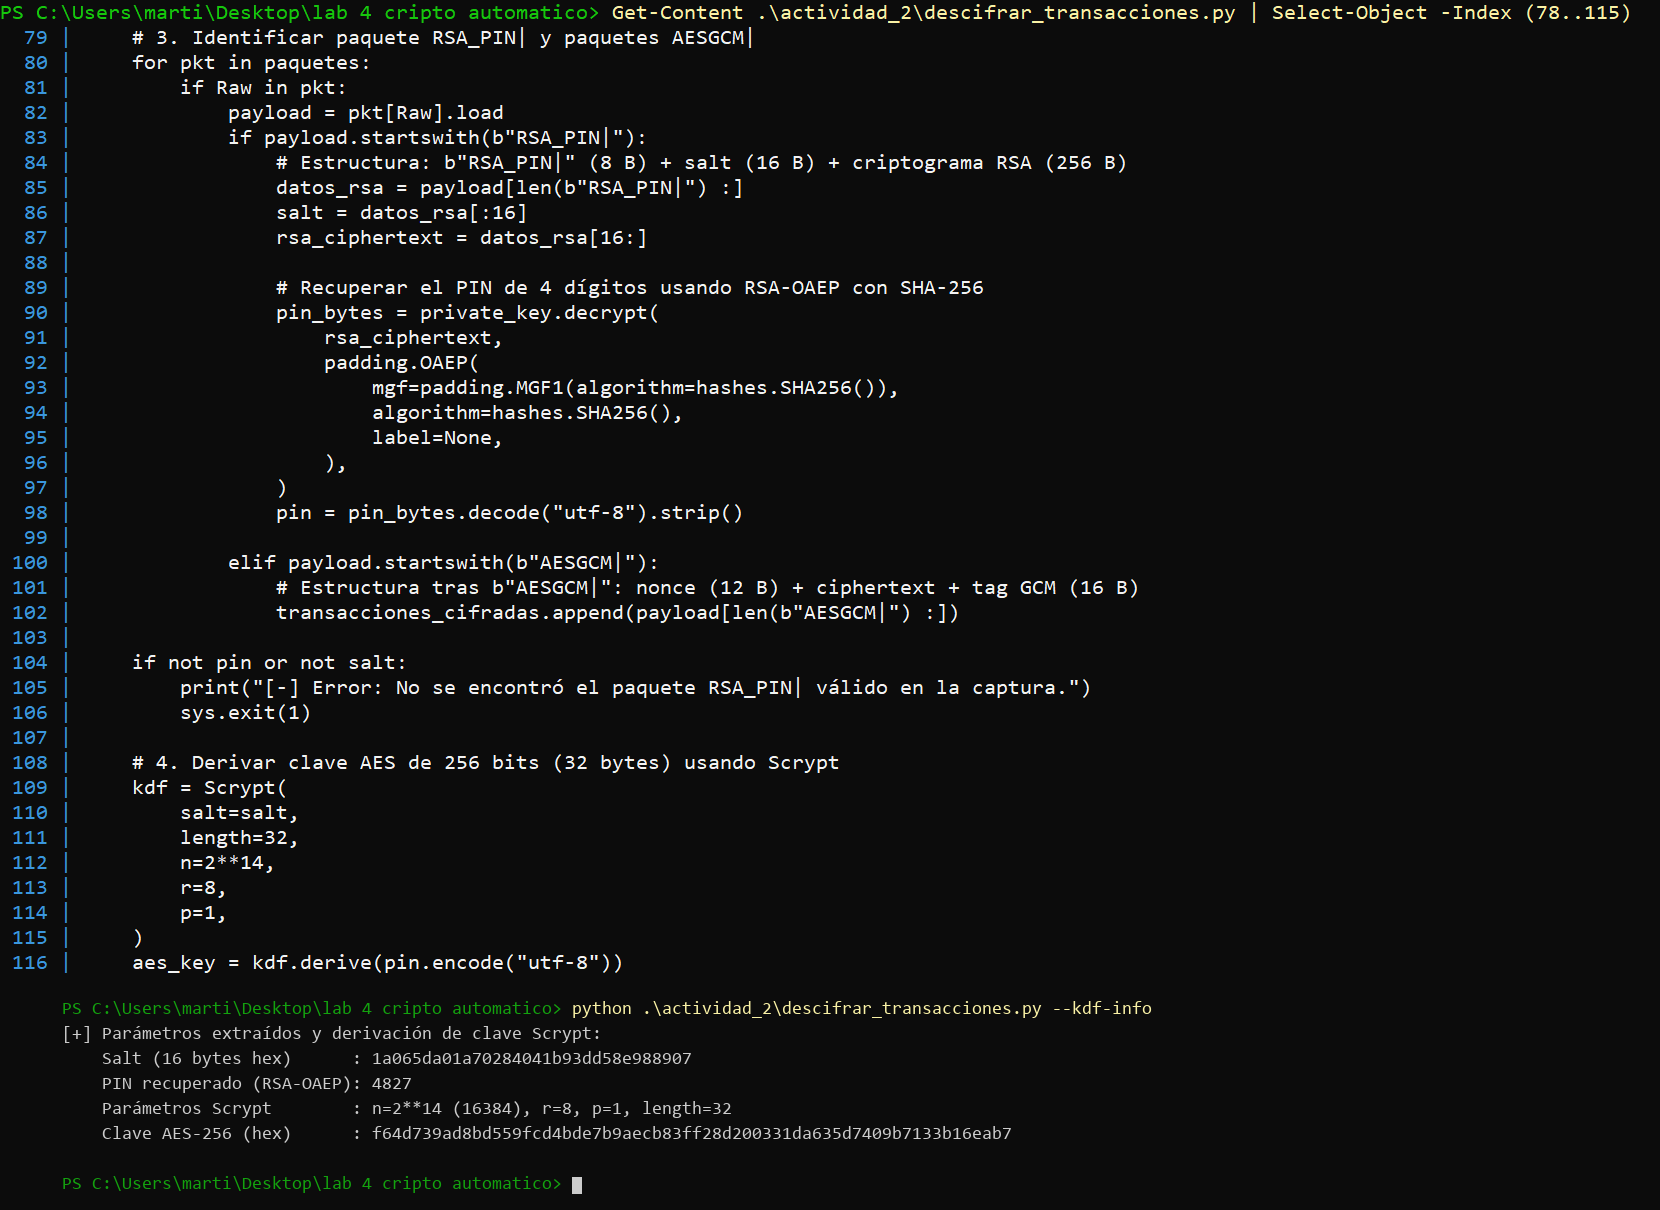
\includegraphics[width=0.98\textwidth]{img/07_codigo_pin_scrypt.png}
    \caption{Sección de código en \texttt{descifrar\_transacciones.py} y ejecución mostrando la \texttt{salt}, el PIN recuperado (\texttt{4827}) y la clave AES-256 derivada.}
    \label{fig:pin_scrypt}
\end{figure}

\noindent\textbf{Función criptográfica de la \texttt{salt} de 16 bytes:}
La \texttt{salt} cumple dos propósitos críticos de seguridad en la derivación de claves basadas en secretos humanos (RFC~7914):
\begin{enumerate}
    \item \textbf{Neutralización de ataques precomputados y tablas arcoíris (\textit{Rainbow Tables}):} Un PIN numérico de 4 dígitos posee un espacio de búsqueda extremadamente reducido de apenas $10^4 = 10{,}000$ valores posibles (\texttt{0000} a \texttt{9999}). Sin una \texttt{salt} aleatoria de alta entropía ($2^{128}$ valores posibles con 16 bytes), bastaría precalcular una sola tabla de $10{,}000$ claves derivadas para invertir instantáneamente cualquier sesión. Al incorporar una \texttt{salt} única de 128 bits, cualquier tabla precomputada queda inutilizada y un atacante se ve forzado a ejecutar el costo completo de CPU y memoria de \texttt{Scrypt} desde cero para cada \texttt{salt} específica.
    \item \textbf{Aislamiento criptográfico entre sesiones:} Incluso si el usuario o sistema reutiliza el mismo PIN (\texttt{4827}) en múltiples sesiones de transferencia, una \texttt{salt} aleatoria diferente en cada sesión garantiza que la clave AES-256 resultante sea completamente distinta e incorrelacionada, evitando colisiones de pares $(\text{clave}, \text{nonce})$ en AES-GCM.
\end{enumerate}

\noindent\textbf{¿Por qué es estrictamente necesario utilizar los mismos parámetros \texttt{(n=2**14)}, \texttt{(r=8)} y \texttt{(p=1)} para obtener la clave AES original?}
\texttt{Scrypt} es una función determinista endurecida en memoria (\textit{memory-hard KDF}, RFC~7914) cuya transformación matemática depende estructuralmente de sus tres parámetros de costo:
\begin{itemize}
    \item $n = 2^{14} = 16{,}384$ define el factor de costo de CPU/memoria (número de iteraciones e instancias de vectores almacenados en RAM durante \texttt{ROMix}).
    \item $r = 8$ fija el tamaño de bloque interno ($128 \cdot r = 1{,}024$ bytes por vector en \texttt{BlockMix}, consumiendo en total $128 \cdot n \cdot r = 16\text{ MiB}$ de memoria secuencial).
    \item $p = 1$ establece el factor de paralelización (cantidad de cadenas independientes \texttt{SMix} generadas por \texttt{PBKDF2-HMAC-SHA256} antes de la mezcla final).
\end{itemize}
Internamente, \texttt{Scrypt} aplica \texttt{PBKDF2-HMAC-SHA256} para expandir $(\text{PIN}, \text{salt})$ en $p$ bloques de $128r$ bytes, ejecuta $n$ rondas de mezcla con la función de núcleo \texttt{Salsa20/8} sobre cada bloque y finalmente vuelve a comprimir la salida con \texttt{PBKDF2-HMAC-SHA256}. Debido al \textbf{efecto avalancha} de las primitivas criptográficas subyacentes, alterar cualquiera de los parámetros ($n$, $r$ o $p$) modifica la geometría de los bloques o la cantidad de rondas de mezcla, produciendo una secuencia de 256 bits estadísticamente independiente de la clave original del emisor. Si se intenta emplear dicha clave errónea en \texttt{AESGCM.decrypt()}, el cálculo del polinomio autenticador \texttt{GHASH} no coincidirá con el \textit{Authentication Tag} de 16 bytes presente en cada paquete, provocando una excepción inmediata (\texttt{InvalidTag}) y haciendo imposible recuperar el texto plano.

\subsubsection{Descifrar los mensajes}

Con la clave AES de 256 bits derivada, el script \href{https://github.com/minicoast/lab4-criptografia-udp/blob/main/actividad_2/descifrar_transacciones.py}{\texttt{actividad\_2/descifrar\_transacciones.py}} inicializa \texttt{AESGCM(aes\_key)} y recorre secuencialmente los 40 paquetes \texttt{AESGCM|}. Para cada paquete extrae los primeros 12 bytes posteriores al encabezado como \texttt{nonce} y el resto como \texttt{ciphertext} (que incluye los 16 bytes finales del \textit{Authentication Tag}), invocando \texttt{aesgcm.decrypt(nonce, ciphertext, None)}. Esta llamada recalcula internamente la etiqueta \texttt{GHASH} sobre $\text{GF}(2^{128})$ en tiempo constante y verifica la autenticidad e integridad íntegra de cada mensaje antes de retornar los bytes descifrados en UTF-8. Las \textbf{40 transacciones fueron autenticadas y descifradas con éxito sin ningún error de integridad}.

\begin{lstlisting}[language=Python,caption={Script completo \texttt{actividad\_2/descifrar\_transacciones.py}.}]
#!/usr/bin/env python3
"""
Laboratorio 4 - Criptografía y Seguridad en Redes
Actividad 2: Análisis de Captura .pcap y Descifrado de Transacciones Financieras

Procedimiento criptográfico implementado:
1. Localización del paquete con etiqueta 'RSA_PIN|', extracción de salt (16 bytes)
   y recuperación del PIN de 4 dígitos mediante RSA-OAEP con SHA-256.
2. Derivación de la clave simétrica AES de 256 bits (32 bytes) mediante Scrypt
   con parámetros exactos n = 2**14, r = 8, p = 1.
3. Localización de los 40 paquetes 'AESGCM|', extracción del nonce de 12 bytes
   y descifrado autenticado (AEAD) mediante AES-GCM.
"""

import argparse
import os
import sys
import warnings

warnings.filterwarnings("ignore")

from scapy.all import rdpcap, Raw
from cryptography.hazmat.primitives import hashes, serialization
from cryptography.hazmat.primitives.asymmetric import padding
from cryptography.hazmat.primitives.kdf.scrypt import Scrypt
from cryptography.hazmat.primitives.ciphers.aead import AESGCM


def resolver_ruta(archivo: str) -> str:
    """Resuelve rutas relativas tanto desde la raíz del proyecto como desde actividad_2/."""
    base_dir = os.path.dirname(os.path.abspath(__file__))
    rutas_posibles = [
        archivo,
        os.path.join(base_dir, "..", archivo),
        os.path.join(base_dir, archivo),
    ]
    for ruta in rutas_posibles:
        if os.path.exists(ruta):
            return os.path.normpath(ruta)
    return archivo


def main():
    parser = argparse.ArgumentParser(
        description="Descifra las transacciones financieras de transacciones_cifradas.pcap"
    )
    parser.add_argument(
        "--kdf-info",
        action="store_true",
        help="Muestra parámetros intermedios (salt en hex, PIN y clave AES-256 derivada)",
    )
    args = parser.parse_args()

    ruta_pcap = resolver_ruta("transacciones_cifradas.pcap")
    ruta_privkey = resolver_ruta("clave_privada.pem")

    if not os.path.exists(ruta_pcap):
        print(f"[-] Error: Archivo de captura no encontrado: {ruta_pcap}")
        sys.exit(1)

    if not os.path.exists(ruta_privkey):
        print(f"[-] Error: Clave privada RSA no encontrada: {ruta_privkey}")
        sys.exit(1)

    # 1. Cargar clave privada RSA-2048 desde formato PEM
    with open(ruta_privkey, "rb") as key_file:
        private_key = serialization.load_pem_private_key(
            key_file.read(),
            password=None,
        )

    # 2. Leer paquetes de la captura de red
    paquetes = rdpcap(ruta_pcap)

    pin = None
    salt = None
    transacciones_cifradas = []

    # 3. Identificar paquete RSA_PIN| y paquetes AESGCM|
    for pkt in paquetes:
        if Raw in pkt:
            payload = pkt[Raw].load
            if payload.startswith(b"RSA_PIN|"):
                # Estructura: b"RSA_PIN|" (8 B) + salt (16 B) + criptograma RSA (256 B)
                datos_rsa = payload[len(b"RSA_PIN|") :]
                salt = datos_rsa[:16]
                rsa_ciphertext = datos_rsa[16:]

                # Recuperar el PIN de 4 dígitos usando RSA-OAEP con SHA-256
                pin_bytes = private_key.decrypt(
                    rsa_ciphertext,
                    padding.OAEP(
                        mgf=padding.MGF1(algorithm=hashes.SHA256()),
                        algorithm=hashes.SHA256(),
                        label=None,
                    ),
                )
                pin = pin_bytes.decode("utf-8").strip()

            elif payload.startswith(b"AESGCM|"):
                # Estructura tras b"AESGCM|": nonce (12 B) + ciphertext + tag GCM (16 B)
                transacciones_cifradas.append(payload[len(b"AESGCM|") :])

    if not pin or not salt:
        print("[-] Error: No se encontró el paquete RSA_PIN| válido en la captura.")
        sys.exit(1)

    # 4. Derivar clave AES de 256 bits (32 bytes) usando Scrypt
    kdf = Scrypt(
        salt=salt,
        length=32,
        n=2**14,
        r=8,
        p=1,
    )
    aes_key = kdf.derive(pin.encode("utf-8"))

    if args.kdf_info:
        print("[+] Parámetros extraídos y derivación de clave Scrypt:")
        print(f"    Salt (16 bytes hex)      : {salt.hex()}")
        print(f"    PIN recuperado (RSA-OAEP): {pin}")
        print(f"    Parámetros Scrypt        : n=2**14 (16384), r=8, p=1, length=32")
        print(f"    Clave AES-256 (hex)      : {aes_key.hex()}")
        return

    # 5. Inicializar primitiva AEAD AES-GCM con la clave derivada de 256 bits
    aesgcm = AESGCM(aes_key)

    # 6. Construir salida exacta según Figura 1 de la guía oficial
    lineas_salida = [
        "[+] PIN recuperado mediante RSA",
        f"[+] PIN: {pin}",
        f"[+] Transacciones cifradas encontradas: {len(transacciones_cifradas)}",
        "",
        "========== TRANSACCIONES ==========",
        "",
    ]

    for idx, bloque_aes in enumerate(transacciones_cifradas, start=1):
        nonce = bloque_aes[:12]
        ciphertext = bloque_aes[12:]

        # AESGCM.decrypt valida el Authentication Tag de 128 bits antes de retornar el texto plano
        plaintext_bytes = aesgcm.decrypt(nonce, ciphertext, None)
        mensaje = plaintext_bytes.decode("utf-8")

        lineas_salida.append(f"[Transacción {idx}]")
        lineas_salida.append(mensaje)
        if idx < len(transacciones_cifradas):
            lineas_salida.append("")

    salida_final = "\n".join(lineas_salida)
    print(salida_final)

    # Guardar salida íntegra de las 40 transacciones en actividad_2/salida_transacciones_completa.txt
    base_dir = os.path.dirname(os.path.abspath(__file__))
    ruta_salida = os.path.join(base_dir, "salida_transacciones_completa.txt")
    with open(ruta_salida, "w", encoding="utf-8") as f_out:
        f_out.write(salida_final + "\n")


if __name__ == "__main__":
    main()
\end{lstlisting}

\begin{figure}[H]
    \centering
    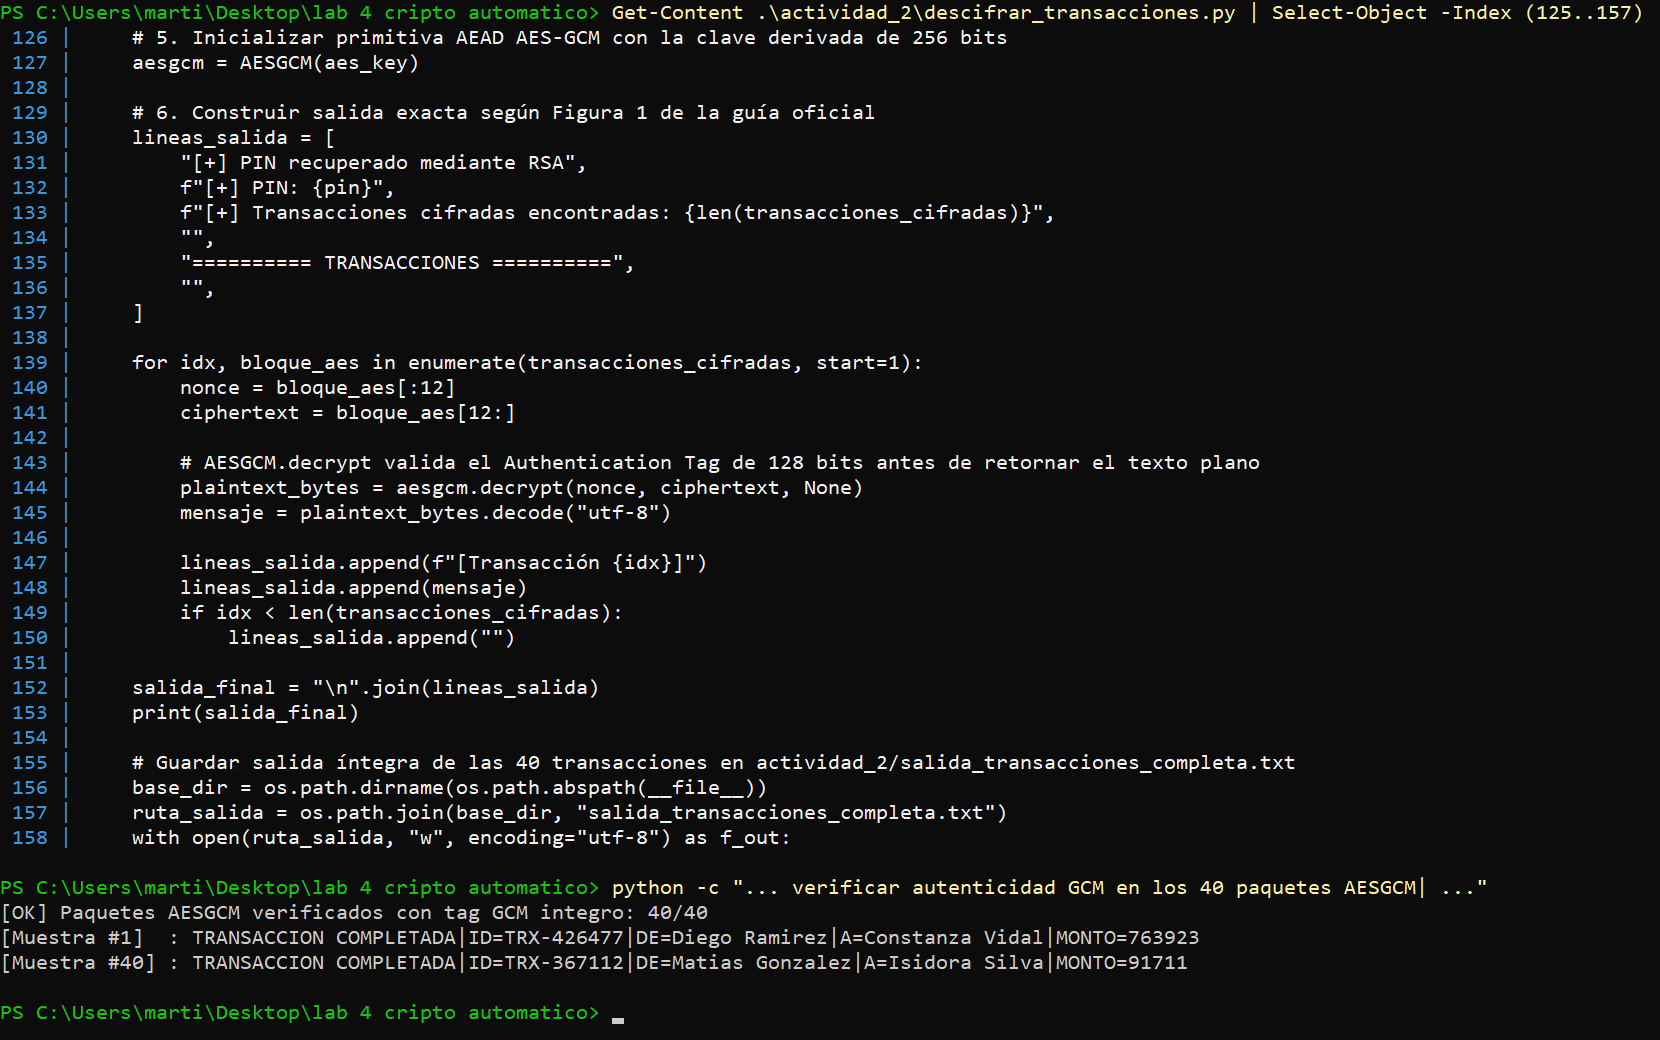
\includegraphics[width=0.98\textwidth]{img/08_codigo_aesgcm.png}
    \caption{Implementación en Python de la extracción del \texttt{nonce} de 12 bytes y verificación autenticada con \texttt{AESGCM.decrypt()}.}
    \label{fig:codigo_aesgcm}
\end{figure}

\begin{figure}[H]
    \centering
    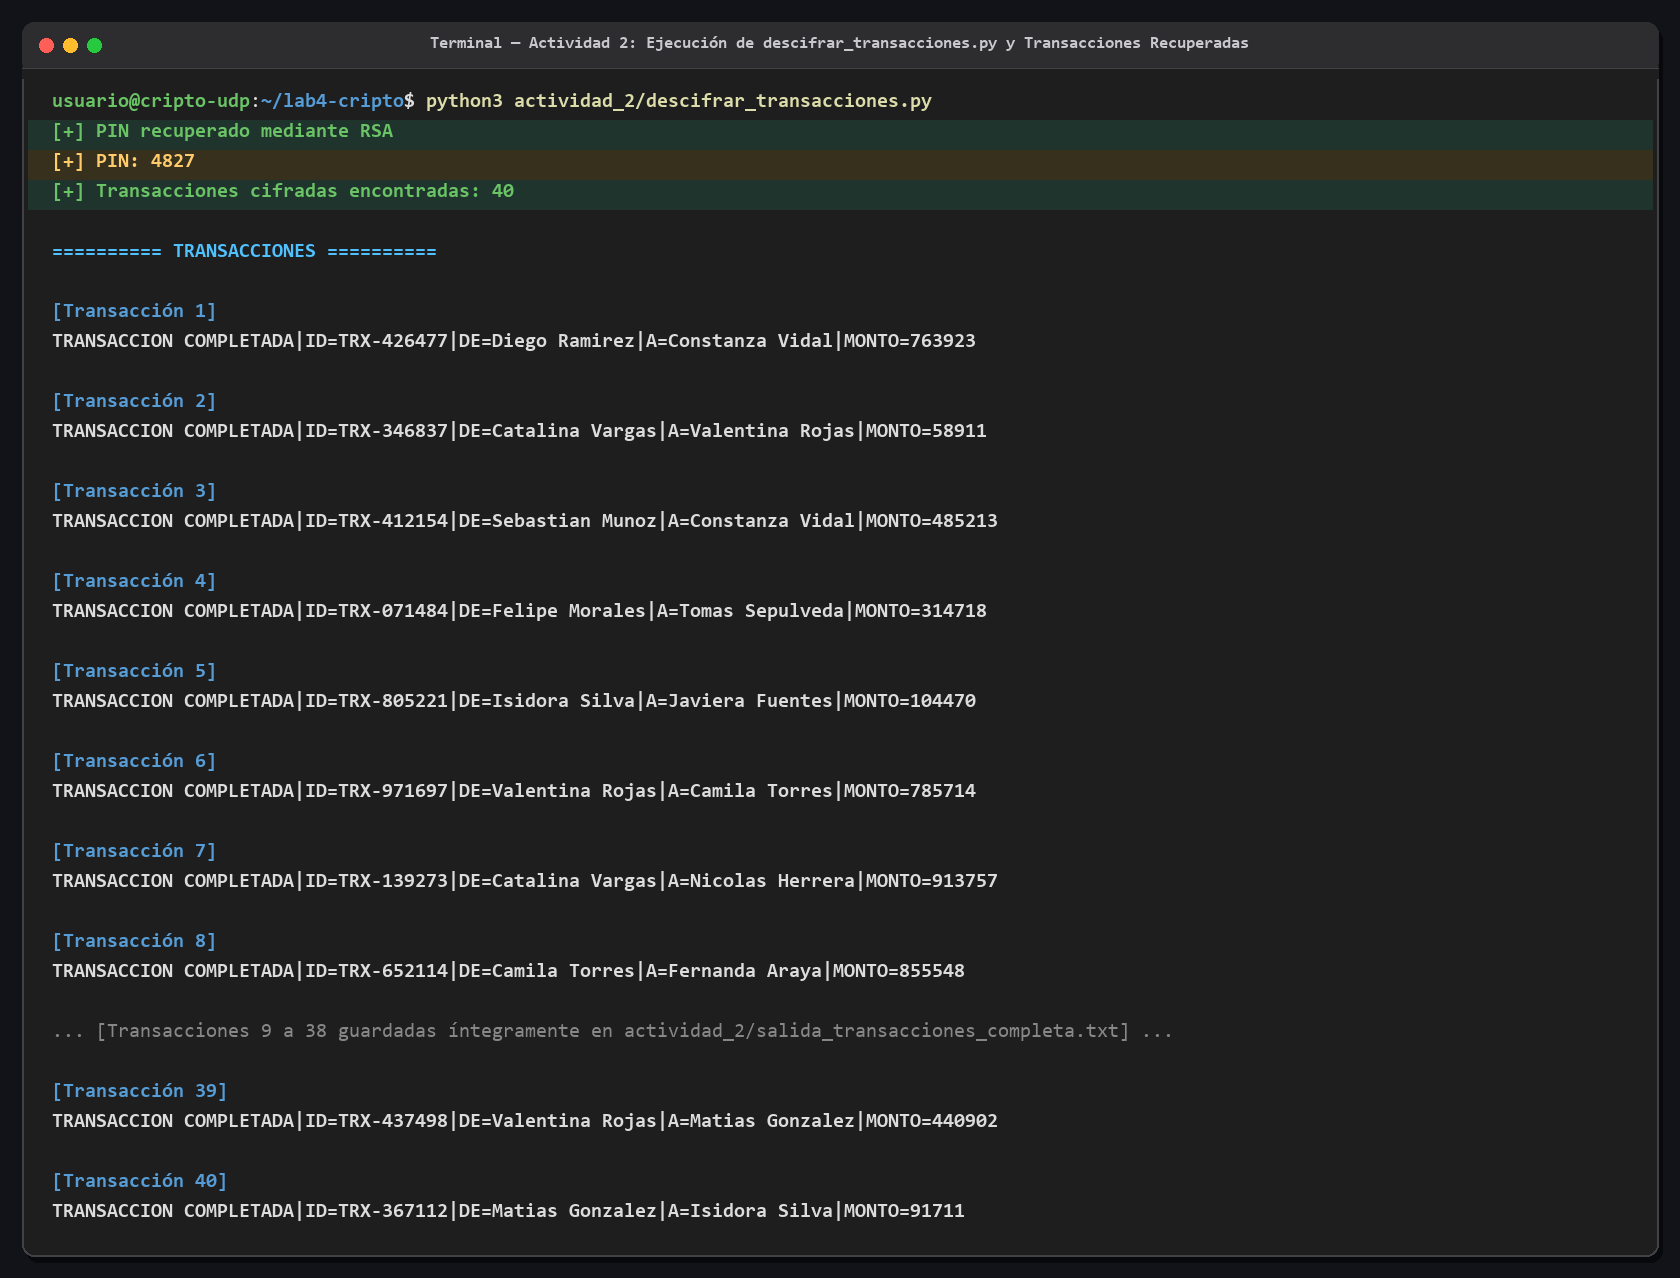
\includegraphics[width=0.98\textwidth]{img/09_resultado_transacciones.png}
    \caption{Ejecución de \texttt{descifrar\_transacciones.py} mostrando el PIN recuperado y las transacciones descifradas en el formato exigido.}
    \label{fig:resultado_transacciones}
\end{figure}

En la Tabla~\ref{tab:transacciones_completas} se presentan las \textbf{40 transacciones financieras recuperadas} con su identificador (\texttt{ID}), remitente (\texttt{DE}), destinatario (\texttt{A}) y monto (\texttt{MONTO}). El archivo de salida íntegro también puede consultarse directamente en \href{https://github.com/minicoast/lab4-criptografia-udp/blob/main/actividad_2/salida_transacciones_completa.txt}{\texttt{actividad\_2/salida\_transacciones\_completa.txt}}.

{\small
\begin{longtable}{@{}rlllr@{}}
\caption{Registro íntegro de las 40 transacciones financieras descifradas y autenticadas.} \label{tab:transacciones_completas} \\
\toprule
\textbf{N\textordmasculine{}} & \textbf{Identificador (ID)} & \textbf{Remitente (DE)} & \textbf{Destinatario (A)} & \textbf{Monto} \\
\midrule
\endfirsthead
\multicolumn{5}{c}{{\tablename\ \thetable{} -- Continuación de la página anterior}} \\
\toprule
\textbf{N\textordmasculine{}} & \textbf{Identificador (ID)} & \textbf{Remitente (DE)} & \textbf{Destinatario (A)} & \textbf{Monto} \\
\midrule
\endhead
\midrule
\multicolumn{5}{r}{{\footnotesize Continúa en la página siguiente...}} \\
\endfoot
\bottomrule
\endlastfoot
1 & \texttt{TRX-426477} & Diego Ramirez & Constanza Vidal & \$763.923 \\
2 & \texttt{TRX-346837} & Catalina Vargas & Valentina Rojas & \$58.911 \\
3 & \texttt{TRX-412154} & Sebastian Munoz & Constanza Vidal & \$485.213 \\
4 & \texttt{TRX-071484} & Felipe Morales & Tomas Sepulveda & \$314.718 \\
5 & \texttt{TRX-805221} & Isidora Silva & Javiera Fuentes & \$104.470 \\
6 & \texttt{TRX-971697} & Valentina Rojas & Camila Torres & \$785.714 \\
7 & \texttt{TRX-139273} & Catalina Vargas & Nicolas Herrera & \$913.757 \\
8 & \texttt{TRX-652114} & Camila Torres & Fernanda Araya & \$855.548 \\
9 & \texttt{TRX-432361} & Vicente Soto & Matias Gonzalez & \$818.686 \\
10 & \texttt{TRX-818929} & Antonia Castro & Tomas Sepulveda & \$885.868 \\
11 & \texttt{TRX-871181} & Catalina Vargas & Camila Torres & \$514.444 \\
12 & \texttt{TRX-157566} & Tomas Sepulveda & Javiera Fuentes & \$436.301 \\
13 & \texttt{TRX-186243} & Vicente Soto & Daniela Reyes & \$698.110 \\
14 & \texttt{TRX-121024} & Isidora Silva & Sebastian Munoz & \$623.481 \\
15 & \texttt{TRX-339097} & Matias Gonzalez & Constanza Vidal & \$77.226 \\
16 & \texttt{TRX-663549} & Isidora Silva & Antonia Castro & \$576.901 \\
17 & \texttt{TRX-367001} & Fernanda Araya & Tomas Sepulveda & \$282.567 \\
18 & \texttt{TRX-188807} & Camila Torres & Antonia Castro & \$195.173 \\
19 & \texttt{TRX-096936} & Felipe Morales & Antonia Castro & \$359.917 \\
20 & \texttt{TRX-695623} & Catalina Vargas & Nicolas Herrera & \$619.299 \\
21 & \texttt{TRX-407749} & Camila Torres & Sebastian Munoz & \$182.369 \\
22 & \texttt{TRX-069658} & Valentina Rojas & Javiera Fuentes & \$556.520 \\
23 & \texttt{TRX-232469} & Felipe Morales & Tomas Sepulveda & \$23.769 \\
24 & \texttt{TRX-940466} & Vicente Soto & Fernanda Araya & \$292.293 \\
25 & \texttt{TRX-755002} & Matias Gonzalez & Daniela Reyes & \$946.989 \\
26 & \texttt{TRX-962321} & Felipe Morales & Daniela Reyes & \$589.780 \\
27 & \texttt{TRX-324981} & Diego Ramirez & Daniela Reyes & \$971.045 \\
28 & \texttt{TRX-337011} & Antonia Castro & Felipe Morales & \$777.198 \\
29 & \texttt{TRX-995006} & Vicente Soto & Sebastian Munoz & \$587.590 \\
30 & \texttt{TRX-630572} & Camila Torres & Sebastian Munoz & \$332.702 \\
31 & \texttt{TRX-517969} & Catalina Vargas & Daniela Reyes & \$484.770 \\
32 & \texttt{TRX-447236} & Matias Gonzalez & Constanza Vidal & \$331.352 \\
33 & \texttt{TRX-852645} & Constanza Vidal & Felipe Morales & \$343.065 \\
34 & \texttt{TRX-188241} & Camila Torres & Constanza Vidal & \$781.107 \\
35 & \texttt{TRX-713923} & Diego Ramirez & Catalina Vargas & \$21.358 \\
36 & \texttt{TRX-362125} & Camila Torres & Sebastian Munoz & \$154.118 \\
37 & \texttt{TRX-961549} & Felipe Morales & Sebastian Munoz & \$614.169 \\
38 & \texttt{TRX-965060} & Tomas Sepulveda & Antonia Castro & \$778.912 \\
39 & \texttt{TRX-437498} & Valentina Rojas & Matias Gonzalez & \$440.902 \\
40 & \texttt{TRX-367112} & Matias Gonzalez & Isidora Silva & \$91.711 \\
\end{longtable}
}

\noindent\textbf{Análisis final sobre Criptografía Post-Cuántica (PQC): ¿Sería posible descifrar los mensajes capturados utilizando las claves pública y privada RSA en cifrados PQC?}

\textbf{Respuesta: NO, no sería posible}, debido a razones fundamentales tanto de \textbf{incompatibilidad matemática y estructural de las primitivas} como del \textbf{modelo de amenaza cuántica}:

\begin{enumerate}
    \item \textbf{Incompatibilidad matemática, algebraica y estructural de claves y algoritmos:}
    Las claves proporcionadas (\texttt{clave\_publica.pem} y \texttt{clave\_privada.pem}) pertenecen al criptosistema \textbf{RSA-2048}, definido sobre aritmética modular en el anillo de enteros $\mathbb{Z}_N$, donde la clave pública es el par $(N, e)$ con módulo compuesto $N = p \cdot q$ de 2048 bits y exponente público $e = 65537$, mientras que la clave privada contiene el exponente privado $d \equiv e^{-1} \pmod{\lambda(N)}$ (cuya seguridad radica en la dificultad clásica de factorizar enteros grandes). Por el contrario, los mecanismos estandarizados en \textbf{Criptografía Post-Cuántica (PQC)} por el NIST —tales como \textbf{ML-KEM / CRYSTALS-Kyber (NIST FIPS~203)} para encapsulamiento de claves o \textbf{ML-DSA / CRYSTALS-Dilithium (NIST FIPS~204)} para firmas digitales— se fundamentan en problemas geométricos y algebraicos completamente distintos, principalmente \textbf{retículos algebraicos estructurados} (\textit{Module Learning With Errors}, MLWE, sobre el anillo polinomial $R_q = \mathbb{Z}_q[X]/(X^{256}+1)$ con $q = 3329$), códigos correctores de errores o árboles de funciones hash. En ML-KEM, una clave privada es un vector de polinomios secretos de coeficientes pequeños $\mathbf{s} \in R_q^k$ y un criptograma es un par de estructuras polinomiales comprimidas $(\mathbf{u}, v)$ producidas añadiendo vectores de ruido acotado. En consecuencia, una clave RSA carece de sentido algebraico, dimensional y de formato dentro de un algoritmo de desencapsulación PQC (\texttt{ML-KEM.Decaps}): ni las claves RSA sirven para abrir mensajes cifrados con PQC, ni un algoritmo PQC puede utilizarse para procesar el criptograma RSA-OAEP de esta captura.

    \item \textbf{Modelo de amenaza cuántica y vulnerabilidad \textit{Harvest Now, Decrypt Later}:}
    El propósito mismo de los algoritmos PQC es reemplazar por completo a RSA y ECC (Curve25519/Ed25519), ya que un computador cuántico tolerante a fallos ejecutando el \textbf{algoritmo de Shor} factoriza el módulo RSA $N$ en tiempo polinomial $\mathcal{O}((\log N)^3)$. Esto significa que un adversario cuántico que haya capturado \texttt{transacciones\_cifradas.pcap} y conozca únicamente \texttt{clave\_publica.pem} podría derivar matemáticamente la clave privada RSA, descifrar \texttt{RSA\_PIN|} para obtener el PIN \texttt{4827}, derivar la clave AES-256 con \texttt{Scrypt} y exponer las 40 transacciones (a pesar de que la capa simétrica AES-256 conserva $\approx 128$ bits de seguridad efectiva frente al algoritmo cuántico de Grover, el eslabón vulnerable es el encapsulamiento asimétrico RSA-2048). Para proteger estas transacciones en un entorno post-cuántico es obligatorio generar un par de claves completamente nuevo nativo de un estándar PQC (por ejemplo, encapsular una semilla aleatoria de 256 bits con \textbf{ML-KEM-768}), prescindiendo totalmente de claves RSA.
\end{enumerate}

% ==================== CONCLUSIONES Y COMENTARIOS ====================
\section*{Conclusiones y comentarios}
\addcontentsline{toc}{section}{Conclusiones y comentarios}

El desarrollo integral de este laboratorio permitió contrastar en la práctica dos paradigmas complementarios de la seguridad de redes moderna: la protección de sesiones interactivas en tránsito mediante \textbf{OpenSSH endurecido} y el análisis criptográfico de un esquema híbrido \textbf{RSA-OAEP + Scrypt + AES-GCM} sobre tráfico capturado.

En la Actividad~1 se comprobó experimentalmente mediante Docker y Wireshark que, aunque SSHv2 expone inevitablemente metadatos de negociación en texto claro durante su fase inicial (banners de software, listas de algoritmos en \texttt{SSH\_MSG\_KEXINIT}, claves públicas y tamaños de paquetes), la combinación explícita de \texttt{curve25519-sha256}, \texttt{ssh-ed25519}, \texttt{aes256-ctr} y \texttt{hmac-sha2-256} establece un canal robusto con autenticación contra ataques \textit{Man-in-the-Middle}, confidencialidad fuerte, integridad por paquete y \textit{Perfect Forward Secrecy} a partir de \texttt{SSH\_MSG\_NEWKEYS}.

En la Actividad~2 se demostró cómo la criptografía híbrida combina el transporte asimétrico del secreto inicial (RSA-2048 con relleno probabilístico OAEP-SHA256) con funciones derivadoras endurecidas en memoria (\texttt{Scrypt} con \texttt{salt} de 128 bits) y cifrado autenticado \texttt{AES-256-GCM}, logrando recuperar y autenticar exitosamente las 40 transacciones financieras. Finalmente, el análisis post-cuántico evidenció tanto la incompatibilidad algebraica absoluta entre claves enteras RSA y primitivas reticulares PQC (como ML-KEM, FIPS~203) como la urgencia de migrar los mecanismos de establecimiento de claves hacia estándares resistentes al algoritmo de Shor para prevenir ataques de captura presente y descifrado futuro (\textit{Harvest Now, Decrypt Later}).

% ==================== 4. BIBLIOGRAFIA ====================
\section{Bibliografia}

\begin{enumerate}
    \item Ylonen, T., \& Lonvick, C. (2006). \textit{The Secure Shell (SSH) Protocol Architecture} (RFC 4251). Internet Engineering Task Force (IETF). \url{https://datatracker.ietf.org/doc/html/rfc4251}
    \item Ylonen, T., \& Lonvick, C. (2006). \textit{The Secure Shell (SSH) Authentication Protocol} (RFC 4252). Internet Engineering Task Force (IETF). \url{https://datatracker.ietf.org/doc/html/rfc4252}
    \item Ylonen, T., \& Lonvick, C. (2006). \textit{The Secure Shell (SSH) Transport Layer Protocol} (RFC 4253). Internet Engineering Task Force (IETF). \url{https://datatracker.ietf.org/doc/html/rfc4253}
    \item Adamantiadis, A., Josefsson, S., \& Baushke, M. (2020). \textit{Secure Shell (SSH) Key Exchange Method Using Curve25519 and Curve448} (RFC 8731). Internet Engineering Task Force (IETF). \url{https://datatracker.ietf.org/doc/html/rfc8731}
    \item Harris, B., \& Velvindron, L. (2020). \textit{Ed25519 and Ed448 Public Key Algorithms for the Secure Shell (SSH) Protocol} (RFC 8709). Internet Engineering Task Force (IETF). \url{https://datatracker.ietf.org/doc/html/rfc8709}
    \item Percival, C., \& Josefsson, S. (2016). \textit{The scrypt Password-Based Key Derivation Function} (RFC 7914). Internet Engineering Task Force (IETF). \url{https://datatracker.ietf.org/doc/html/rfc7914}
    \item Dworkin, M. (2007). \textit{Recommendation for Block Cipher Modes of Operation: Galois/Counter Mode (GCM) and GMAC} (NIST Special Publication 800-38D). National Institute of Standards and Technology. \url{https://doi.org/10.6028/NIST.SP.800-38D}
    \item National Institute of Standards and Technology [NIST]. (2024). \textit{Module-Lattice-Based Key-Encapsulation Mechanism Standard (ML-KEM)} (FIPS PUB 203). U.S. Department of Commerce. \url{https://doi.org/10.6028/NIST.FIPS.203}
\end{enumerate}

\vspace{0.4cm}
\begin{itemize}
    \item \textbf{Captura y Claves:} La totalidad de las evidencias experimentales del laboratorio —incluyendo las capturas de red (\href{https://github.com/minicoast/lab4-criptografia-udp/blob/main/actividad_1/captura_ssh.pcap}{\texttt{captura\_ssh.pcap}} y \href{https://github.com/minicoast/lab4-criptografia-udp/blob/main/transacciones_cifradas.pcap}{\texttt{transacciones\_cifradas.pcap}}), el par de claves RSA (\href{https://github.com/minicoast/lab4-criptografia-udp/blob/main/clave_publica.pem}{\texttt{clave\_publica.pem}} y \href{https://github.com/minicoast/lab4-criptografia-udp/blob/main/clave_privada.pem}{\texttt{clave\_privada.pem}}), los archivos \href{https://github.com/minicoast/lab4-criptografia-udp/blob/main/actividad_1/Dockerfile}{\texttt{Dockerfile}} y \href{https://github.com/minicoast/lab4-criptografia-udp/blob/main/actividad_1/sshd_config}{\texttt{sshd\_config}}, los scripts en Python (\href{https://github.com/minicoast/lab4-criptografia-udp/blob/main/actividad_2/analizar_pcap.py}{\texttt{analizar\_pcap.py}} y \href{https://github.com/minicoast/lab4-criptografia-udp/blob/main/actividad_2/descifrar_transacciones.py}{\texttt{descifrar\_transacciones.py}}), los registros íntegros de consola y las 40 transacciones descifradas— se encuentran disponibles públicamente en el repositorio oficial de GitHub:\\
    \href{https://github.com/minicoast/lab4-criptografia-udp}{\texttt{https://github.com/minicoast/lab4-criptografia-udp}}
\end{itemize}

\end{document}
